\documentclass[UTF8,11pt,oneside]{ctexbook}
\newcommand{\bookname}{数学物理方程}
\newcommand{\uira}{https://github.com/ZhangtongCN}
\newcommand{\uirb}{https://github.com/Clignniis}
%数学符号
\usepackage{amsmath,amssymb,amsfonts,esint,mathrsfs}
\usepackage{tikz}
%合并单元格
\usepackage{multirow}
\usepackage{geometry}
%三线表
\usepackage{booktabs}
%\usepackage[toc]{multitoc}%双栏目录
%颜色设置
\usepackage{xcolor}
\definecolor{nuist}{RGB}{0, 103, 156}%南信大蓝
\definecolor{sky}{RGB}{101, 170, 221}%天空蓝
\definecolor{tech}{RGB}{38, 96, 173}%科技蓝
\definecolor{gold}{RGB}{201, 160, 99}%高贵金
%引用
\usepackage[colorlinks]{hyperref}
%设置页眉页脚

%章节设置
\ctexset{
    %chapter={pagestyle=fancy},%使得章节页页眉页脚格式一致
}
\geometry{a4paper,top=2.5cm,bottom=2.5cm}
\setcounter{tocdepth}{1}
\linespread{1.3}\selectfont

%页眉页脚
\usepackage{fancyhdr}
\pagestyle{fancy}
\renewcommand{\sectionmark}[1]{\markright{\thesection\ #1}}
\fancyhf{}
\fancyhead[L]{\href{https://github.com/ZhangtongCN}{\textcolor{tech}{\bookname}}}
\fancyhead[R]{\href{https://github.com/ZhangtongCN}{\textcolor{tech}{笔记整理与汇总}}}
\fancyfoot[C]{\href{https://github.com/Clignniis}{\textcolor{tech}{\thepage}}}
\renewcommand{\headrulewidth}{0pt}
\setlength{\headheight}{27pt}

\begin{document}

\frontmatter

\begin{titlepage}
    \begin{tikzpicture}[remember picture, overlay]
        \node at ([shift={(0,1)}]current page.center){
            \begin{tikzpicture}[scale=0.7]
            \path[fill=sky] (0:0)--++(90:2)--++(30:6)--++(150:6)--++(210:6)--++(330:6)--++(90:1)--++(150:4)--++(30:4)--++(330:4)--++(210:4)--++(270:3)--++(150:1)--++(210:3)--++(270:1)--++(30:5)--++(330:3)--++(270:1)--++(210:4)--++(150:4)--++(210:1)--++(330:5)--++(30:5)--cycle;
            \path[fill=cyan!50] (0:0)--++(270:1)--++(210:3)--++(150:1)--++(90:5)--++(150:1)--++(270:6)--++(30:6)--++(90:1)--++(30:4)--++(270:6)--++(210:5)--++(270:1)--++(30:6)--++(90:8)--++(210:6)--cycle;
            \path[fill=cyan!50] (90:6)--++(90:1)--++(210:4)--++(330:1)--++(30:3)--++(90:1);
            \path[fill=nuist] (0:0)--++(270:1)--++(330:3)--++(30:1)--++(90:5)--++(30:1)--++(270:6)--++(150:6)--++(90:1)--++(150:4)--++(270:6)--++(330:5)--++(270:1)--++(150:6)--++(90:8)--++(330:6)--cycle;
            \path[fill=nuist] (90:6)--++(90:1)--++(330:4)--++(210:1)--++(150:3)--++(90:1);
            \end{tikzpicture}
        };
        \node[gold] at ([shift={(0,8)}]current page.center){\fontsize{72}{0}\heiti \bookname};
        \node at ([shift={(0,-5)}]current page.center){\Huge\heiti\href{\uira}{\textcolor{nuist}{Tong Zhang}}\quad\href{\uirb}{\textcolor{nuist}{Cls}}};
        \node[tech, anchor= south] at ([shift={(0,6)}]current page.south){\fontsize{48}{0}\heiti 笔记整理与汇总};
    \end{tikzpicture}
\end{titlepage}

\chapter*{版权声明}

本《\bookname{} 笔记整理与汇总精编版》一册电子版遵循有限的知识共享许可协议。本书授权包含署名-非商业性使用-相同方式共享(CC BY-NC-SA)。即您被允许在授权范围内对该电子书进行转载、节选、二次创作,但不得用于任何商业目的,且使用时须署原作名,且必须采用与本创作相同的协议(CC BY-NC-SA)进行授权。限于编者水平,本书难免有疏漏错误,敬请读者批评指正。

\begin{tikzpicture}[remember picture, overlay]
    \node [opacity=0.4] at (current page.center){
        \begin{tikzpicture}[scale=2]
            \foreach \a/\c in {0/90, 120/80, 240/70} {%
                \path[fill=nuist!\c] (0+\a :2.309)--++(150+\a :5)--++(270+\a :7)--++(150+\a :1)--++(90+\a :8)--++(330+\a :7)--cycle;
            }
        \end{tikzpicture}
    };
\end{tikzpicture}

\tableofcontents

\mainmatter


\chapter{绪论}
 
为方便复习使用,本书中带星号*的内容了解即可

\section{基本概念}

微分方程:有自变量、未知函数以及未知函数的导数或微分的方程。分为常微分方程(ODE,未知函数为一元函数)和偏微分方程(PDE,有未知函数关于自变量的偏导数的等式,即\(F\left(x,y,\ldots,u,u_x,u_y,\ldots,u_{xx},\ldots\right)=0\))

PDE方程组由多个未知函数与多个PDE组成,它的阶是PDE中最高阶偏导数的阶数。最高阶偏导数即为未知函数右下角自变量的个数。

PDE有以下分类:
\begin{enumerate}
	\item 线性PDE	
	\begin{enumerate}
		\item 齐次:方程中无自由项,即没有不含未知函数及偏导数的项。
		\item 非齐次:有自由项,如\(u_{xyy}+u_{yy}+2u=5x\)
	\end{enumerate}
	\item 非线性PDE	
	\begin{enumerate}
		\item 拟线性PDE:关于未知函数的所有最高阶偏导数是线性的,如\(u_xu_{xx}+xuu_y=\sin{3x}\)
		\item 半线性PDE:最高阶偏导的系数不含未知函数而依赖于自变量,如\(u_t+kuu_x+u_{xxx}=0\)
		\item 完全非线性,如\(\left(u_x\right)^2+u=3\)
	\end{enumerate}
\end{enumerate}

方程的求解有:分离变量法、行波法、积分变换法、格林函数法。解的类型分为:古典解,弱解,特解和通解	

典型PDE
\begin{enumerate}
	\item 哈密顿算子(梯度算符)\(\nabla=\left(\frac{\partial}{\partial x_1},\frac{\partial}{\partial x_2},\ldots,\frac{\partial}{\partial x_n}\right)\)需要记住
	\item n维拉普拉斯算子\(\Delta=\nabla\cdot\nabla=\frac{\partial^2}{\partial x_1^2}+\frac{\partial^2}{\partial x_2^2}+\ldots+\frac{\partial^2}{\partial x_n^2}\)
	\item 散度算子:设\(A=P(x,y,z)i+Q(x,y,z)j+R(x,y,z)k,\mathrm{div}A=P_x+Q_y+R_z\)
	\item 散度定理:\(\iint\limits_s A\cdot n\,\mathrm{d}s=\iiint_{V}\mathrm{div}A\,\mathrm{d}v\)
	\item 旋度算子:\(\mathrm{rot}A=\left(R_y-Q_z,P_z-R_x,Q_x-P_y\right)=
	\begin{vmatrix}
		i&j&k\\
		\frac{\partial}{\partial x}&\frac{\partial}{\partial y}&\frac{\partial}{\partial z}\\
		P&Q&R\\
	\end{vmatrix}\)
	\item 关系:\(\mathrm{grad}u=\nabla u\quad\mathrm{div}A=\nabla\cdot A\quad\mathrm{rot}A=\nabla\times A\)

\end{enumerate}

典型方程
\begin{enumerate}
	\item n维波动\(u_{tt}-a^2\Delta u=0\)
	\item 三维热传导\(u_t-a^2\left(u_{xx}+u_{yy}+u_{zz}\right)=0\)
	\item n维拉普拉斯方程\(-\Delta u=0\)
	\item 三维泊松方程\(-\left(u_{xx}+u_{yy}+u_{zz}\right)=f(x,y,z)\)
\end{enumerate}

\section{典型方程的导出*}

\subsection{波动方程}

\subsubsection{问题提出}

有一根长为l的均匀柔软富有弹性的细弦,在外力作用下作微小横振动,确定弦的运动方程

\subsubsection{问题分析}

明确:
\begin{enumerate}
	\item 研究物理量:弦沿垂直方向位移\(u(x,y)\)
	\item 物理定律:牛顿第二定律、胡克定律
	\item 建立范定方程
\end{enumerate}

\subsubsection{模型假设}

\begin{enumerate}
	\item 柔软且有弹性:弦的张力沿弦切线方向,张力大小按照胡克定律,对外力无抵抗性
	\item 细弦:重量与其张力相比很小
	\item 微小振动:位移后斜率\(\approx1 \quad\sin\alpha\approx u_x\)
	\item 横振动:弦运动于二维平面,弦上各点沿垂直\(x\)方向运动
\end{enumerate}

\subsubsection{模型建立(三步骤)}

\begin{enumerate}
	\item 确定物理量与坐标系(微元法)
	\item 证明张力为常数(水平胡克定律)
	\item 导出弦振动方程(竖直方向结合牛二定律)
\end{enumerate}

\subsubsection{推导}

坐标系:考察弦上微小元素,任取一小段\(MM'\),长为\(\Delta x\),\(\rho\)为弦线密度

证明\(T\)为常数:水平方向上,\(T\left(x+\Delta x\right)\cos{\alpha'}=T(x)\cos{\alpha}\)当振幅很小时\(\alpha\approx0\),故\(T\left(x+\Delta x\right)\approx T(x)\)与\(x\)无关。由于弦长未变,\(\Delta s=\int_{x}^{x+\Delta x}{\sqrt{1+u_x^2}\,\mathrm{d}x}\approx\Delta x\)故\(T\)与\(t\)无关。

导出方程:垂直方向上\(T\sin\alpha'-T\sin\alpha+F(x,t)_{\text{外力密度}}\Delta x=\rho\Delta x_{\text{质量}}{u_{tt}}_\text{加速度}\)有\(\sin\alpha'\approx\tan{\alpha'}=u_x(x+\Delta x)\quad\sin\alpha\approx\tan\alpha=u_it{x}(x)\)则:\(T\left[u_x\left(x+\Delta x\right)-u_x(x)\right]+F(x,t)\Delta x=\rho\Delta xu_{tt}\Rightarrow Tu_{xx}+F=\rho u_{tt}\quad u_{tt}=\frac{T}{\rho}u_{xx}+\frac{F}{\rho}\Rightarrow u_{tt}=a^2u_{xx}(x,t)+f(x,t)\)。其中\(a^2=\frac{T}{\rho},f(x,t)=\frac{F(x,t)}{\rho}\)

弦的受迫振动方程
\begin{enumerate}
	\item 自由振动方程:弦上不受外力\(u_{tt}=a^2u_{xx}\)
	\item 高维拓展:二维薄膜\(u_{tt}=a^2\left(u_{xx}+u_{yy}\right)+f(x,y,t)\)、三维声波光波
\end{enumerate}

\subsection{一维热传导方程}

推导过程
\begin{enumerate}
	\item 热能密度:单位体积所受热能量\(e(x,t)\)
	\item 热通量:本质上是有方向的热能量。单位时间向右流过单位面积的热能量。\(\phi(x,t)\)在\(\Delta x\)部分,流入为\(\phi(x,t)\),流出为\(\phi\left(x+\Delta x,t\right)\)
	\item 热源:在单位时间内单位体积生成的热能量\(Q(x,t)\)
	\item 热能守恒定律:\(\frac{\partial\left[A\Delta xe(x,t)\right]}{\partial t}=\phi(x,t)A-\phi\left(x+\Delta x,t\right)A+Q(x,t)A\Delta x\)(使用微分表达,左边为这一段微元体内热能的变化率,右边为流入-流出+热源)\(\frac{\partial e}{\partial t}=\lim_{\Delta x\rightarrow0}{\frac{\phi(x,t)-\phi\left(x+\Delta x,t\right)}{\Delta x}=}-\frac{\partial\phi}{\partial x}+Q\)
	\item 比热:\(c(x)\) 单位变化1℃变化能量
	\item 体积密度:\(\rho(x)\)
	\item 温度:\(u(x,t)\)关系:温度和能量转换定律\(e(x,t)A\Delta x=c(x)u(x,t)\cdot\rho A\Delta x=\rho cu(x,t)\)
	\item 热传导系数:热通量\(\phi=-K_0\frac{\partial u}{\partial x}\)
	\item 傅里叶热传导定律\(\frac{\partial u}{\partial x}\)为梯度,温度在杆上做传导是因为受热不均,\(\frac{\partial u}{\partial x}<0\)则代表温度向\(x\)方向递减,故热量向\(x\)方向传递,故通量有负号。\(\phi\)表示单位时间单位面积上的热流量\(\phi=\frac{\mathrm{d}Q}{\mathrm{d}s\mathrm{d}t}\)由此,可代入原式:\(c\rho\frac{\partial u}{\partial t}=\frac{\partial}{\partial x}\left(K_0\frac{\partial u}{\partial x}\right)+Q\Rightarrow\frac{\partial u}{\partial t}=a^2\frac{\partial^2}u{\partial x^2}+\frac{Q}{c\rho}\quad a=\sqrt{\frac{K_0}{c\rho}}\)
\end{enumerate}
		
\subsection{拉普拉斯方程/泊松方程}
方程描述一种稳定的状态,其不随时间变化,随位置变化
\begin{gather*}
0=a^2\left(\frac{\partial^2u}{\partial x^2}+\frac{\partial^2u}{\partial y^2}+\frac{\partial^2u}{\partial z^2}\right)+f\\
\nabla^2u=f  \nabla^2u=\frac{\partial^2u}{\partial x^2}+\frac{\partial^2u}{\partial y^2}+\frac{\partial^2u}{\partial z^2}
\end{gather*}

\section{定解条件与定解问题*}

描述物理现象需要偏微分方程(泛定方程)+ 定解条件,其中的定解条件为准确说明对象的初始状态以及边界上的约束条件。
	
不同支撑时弦的振动:边界条件不同;在不同位置拨动弦:初始条件不同。即使泛定方程相同,不同的边界条件或初始条件也可能导致完全不同的解。

\subsection{初始条件(说明初始状态的条件)}
柯西(Cauchy)初始条件:用以给出具体物理现象的初始状态。用来演变到未来的初状态。可分为以下三类问题。


\subsubsection{弦振动问题}

初始条件是指弦在开始振动时刻的位移\(f(x)\)和速度\(g(x)\)
\[
\begin{cases}u|_{t=0}=f(x)\\\frac{\partial u}{\partial t}|_{t=0}=g(x)\end{cases}
\]

\subsubsection{热传导问题}

初始条件是指开始传热的时刻物体温度的分布情况,以\(f(x)\)表示\(t=0\)时物体内一点\(x\)的温度\[
u(x,t)|_{t=0}=f(x)
\]

\subsubsection{泊松/拉普拉斯}

描述稳恒状态,与时间无关,所以不提初始条件

\subsubsection{注意}
\begin{enumerate}
	\item 不同类型的方程,相应初值条件的个数不同
	\item 关于\(t\)的\(n\)阶偏微分方程,要给出\(n\)个初始条件
	\item 初始条件给出的应是整个系统的初始状态,而非系统中个别点的初始状态
\end{enumerate}

\subsection{边界条件(说明边界上约束情况的条件)}

\subsubsection{弦振动三大类}
\begin{enumerate}
	\item 固定端\(u\left(L,t\right)=0,t\geq0\)
	\item 可控端点\(u(x,t)|_{x=0}=f(t)\)可选择\(f(t)\),非齐次
	\item 自由端\(T\left.\frac{\partial u}{\partial x}\right|_{x=L}=0\)或者\(u_x\left(L,t\right)=0,t\geq0\)其中\(T\)为张力
	\item 弹性支撑端\((u_x+\sigma u)|_{x=L}=0\)其中\(\sigma=k/T\)为弹性支撑力
\end{enumerate}

\subsubsection{热传导三大类}
\begin{enumerate}
	\item 定温端:物体与外界接触的表面温度已知,\(u(x,y,z,t)=f(x,y,z),(x,y,z)\in\partial\Omega\)
	\item 绝热端:在表面\(S\)上热量的流速始终为0,\(\frac{\partial u}{\partial n}=0,(x,y,z)\in\partial\Omega,t\geq0\)
	\item 热交换端:\((u_n+\sigma u)|_{\partial\Omega}=\sigma u_1\)
\end{enumerate}

\subsubsection{三类边界条件(设\(u\)为未知函数,\(\partial\Omega\)为边界)}
\begin{enumerate}
	\item 第一类边界条件(狄利克雷(Dirichlet)边界条件):直接给出\(u\)在边界\(\partial\Omega\)上的值
	\item 第二类边界条件(诺依曼(Neuman)边界条件):给出\(u\)沿\(\partial\Omega\)的外法线方向的方向
	\item 第三类边界条件(罗宾(Robin)边界条件):给出\(u\)以及\(\frac{\partial u}{\partial n}\)的线性组合在边界的值\(\left.\left(\frac{\partial u}{\partial n}+\sigma u\right)\right|_{\partial\Omega}=f\)
\end{enumerate}
\subsubsection{注意}
\begin{enumerate}
	\item 上面给出的边界条件中,\(f_i(i=1,2,3)\)都是定义在边界\(\partial\Omega\)上的已知函数
	\item 当\(f_i=0\)时,相应的边界条件称为齐次的,否则称为非齐次的
	\item 三种条件可归为一式:\(\left.\left(\alpha\frac{\partial u}{\partial n}+\beta u\right)\right|_{\partial\Omega}=f\begin{cases}
		\alpha=0,\beta\neq0\quad\text{第一类}\\
		\alpha\neq0,\beta=0\quad\text{第二类}\\
		\alpha\neq0,\beta\neq0\quad\text{第三类}
	\end{cases}\)
\end{enumerate}

\subsection{定解条件}

初始条件+边界条件=定解条件,泛定方程+定解条件=定解问题。衔接条件:由于系统由不同介质组成,在两种不同介质的交界处需给定两个衔接条件;其他条件:由于物理上的合理性的需要,有时还需对未知函数附加以单值、有限、周期性等限制,这类附加条件称为自然边界条件。

\subsubsection{初值问题或Cauchy问题:泛定方程+初始条件}

在无穷的区域里面研究的问题

波动方程的柯西问题:\(\begin{cases}u_t-a^2u_{xx}=0,-\infty<x<+\infty,t>0\\
	u|_{t=0}=\phi(x),-\infty<x<+\infty\end{cases}\)

热传导方程的柯西问题:\(\begin{cases}u_{tt}-a^2u_{xx}=0,-\infty<x<\infty,t>0\\
	u|_{t=0}=\phi(x),{u}_t|_{t=0}=\psi(x)-\infty<x<+\infty\end{cases}\)

\subsubsection{边值问题 :泛定方程+边界条件(三类)}

泊松方程的边值问题

第一类:\(\begin{cases}\Delta u=f(x,y,z),(x,y,z)\in\Omega\\u|_{\partial\Omega}=\varphi(x,y,z),(x,y,z)\in\partial\Omega\end{cases}\)

第二类:\(\begin{cases}\Delta u=f(x,y,z),(x,y,z)\in\Omega\\\frac{\partial u}{\partial n}|_{\partial\Omega}=\varphi(x,y,z),(x,y,z)\in\partial\Omega\end{cases}\)

第三类:\(\begin{cases}\Delta u=f(x,y,z),(x,y,z)\in\Omega\\(\frac{\partial u}{\partial n}+\sigma u)|_{\partial\Omega}=\varphi(x,y,z),(x,y,z)\in\partial\Omega\end{cases}\)

\subsubsection{初边值问题:泛定方程+初始条件+边界条件(混合问题)}

一维齐次弦振动方程的混合问题:\(\begin{cases}u_{tt}-a^2u_{xx}=0,0<x<l,t>0\\u|_{t=0}=\phi(x),u_t|_{t=0}=\psi(x),0\le x\le l\\u_x\left(0,t\right)=u_x\left(l,t\right)=0,t\geq0\end{cases}\)

其他定解问题:混合边值问题、外边值问题

\subsection{例题}
\begin{enumerate}
	\item 长为\(l\),\(x=0\)端固定的均匀细杆,处于静止,在\(t=0\)时,一个沿着杆长方向的力\(F\)加在杆的另一端,求\(t>0\)杆上各点位移的定解条件\\
	边界条件:\(u(x,t)|_{x=0}=0\quad\frac{\partial u}{\partial x}|_{x=l}=\frac{F}{ES}\)\\
	初始条件:\(u|_{t=0}=0\quad\frac{\partial u}{\partial t}|t_{t=0}=0\)
	\item 一长为\(L\)初始温度为\(\varphi(x)\)的均匀细杆,其侧表面与周围介质无热交换,内部有密度为\(g(x,t)\)的热源,右端绝热,左端与温度为\(u\)的介质有热交换。试写出杆内温度分布的定解问题。\\
	范定方程:\(\frac{\partial u}{\partial t}=a^2\frac{\partial^2u}{\partial x^2}+\frac{g(x,t)_\text{热源}}{c\rho},0<x<L,t>0\)\\
	初始条件:\(u(x,0)=\varphi(x),0\leq x\leq L\)\\
	边界条件:\(u_x(L,t)=0,K\left.\frac{\partial u}{\partial x}\right|_{x=0}=h(u(0,t)-u)\quad t>0\)
	\item 一长为\(L\)的弹性杆,一端固定,另一端被拉离平衡位置\(b\)长度而静止,放手任其振动,试求杆振动的定解问题。\\
	范定方程:\(u_{tt}=a^2u_{xx}\quad 0<x<L,t>0\)\\
	初始条件:\(u(x,0)=\frac{x}{L}b,u_t(x,0)=0,0\leq x\leq L\)\\
	边界条件:\(u(0,t)=0,u_x(L,t)=0,t\geq0\)
	\item 一边长为\(l\)的正方形薄板如图\ref{pic:sqr},其\(y=0\)边保持恒温\(T\),其他三边保持0℃,求稳恒状态下板内温度的定解问题。\\
	范定方程:\(u_{xx}+u_{yy}=0,0<x,y<l\)\\
	\(x\)边:\(u|_{x=0}=0,u|_{x=l}=0,0\leq y\leq0\)\\
	\(y\)边:\(u|_{y=0}=T,u|_{y=t}=0,0\leq x\leq l\)
\end{enumerate}
\begin{figure}[htbp]
	\centering
	\begin{tikzpicture}[>=latex]
		\draw[->](-0.2,0)--(2.2,0)node[right]{\(x\)};
		\draw[->](0,-0.2)--(0,2.2)node[above]{\(y\)};
		\node at(-0.2,-0.2){\(O\)};
		\draw(0,2)node[left]{\(l\)}--(2,2)--(2,0)node[below]{\(l\)};
	\end{tikzpicture}
	\caption{正方形薄板}\label{pic:sqr}
\end{figure}

\section{定解问题的适定性}

研究提法的合理性,要求满足:存在性(是否有解),唯一性(是否有唯一解),稳定性(解是否连续依赖定解条件(定解条件有微小变动时,引起解的变动是否足够小)。当条件过多时,可能无解;条件过少,可能解不唯一;条件不恰当,可能解不稳定。

\subsection{定解问题的解*}
\begin{enumerate}
	\item 定解问题的解:在指定的范围内满足方程,同时满足所给的定解条件的函数
	\item 古典解:具有方程中出现的各个偏导数且一般说它们应该是连续的以保证函数可微的解
	\item 弱解(物理解):函数在个别的点(线、面)上不可导或导数不连续,其不满足古典解的要求,但其在实际问题中是有意义的 。写出弱形式的方程进行求解得到弱解(有限元数值求解)
\end{enumerate}

\subsection{定解问题的适定性}

实际问题中,如果一定解问题的解存在、唯一、稳定,则称其适定的(well-posed),否则,称其为不适定的(ill-posed)。	适定性的讨论对于检查定解问题是否能在允许范围内真实地反映所对应的实际问题常常是有效的。先考虑适定性,有助于发现建立的数学模型是否存在失误。

不适定问题的例子:拉普拉斯方程的初值仅仅只有微小扰动,最终值却发生极大的变化,因此该问题不适定,拉普拉斯方程只提边界条件。

\section{线性叠加原理}

\subsection{引入*}

\subsubsection{叠加原理}

物理学解释:几种不同原因综合产生的效果等于这些原因单独产生效果的累加。例如力的叠加原理、电场的叠加原理、电势叠加原理(标量、向量场均有叠加原理)。

\subsubsection{思考问题}

叠加原理存在性、其表现形式、应用。

\subsubsection{线性PDE叠加原理}
\begin{enumerate}
	\item 适用条件:泛定方程、定解条件都是线性的:线性定解问题 (对于线性,叠加原理是普适的)
	\item 数学表达:将复杂的定解问题看作是若个相对简单部分的线性叠加而成,这几个部分所得出的解的线性叠加给出的形式解,即为原定解问题的解 (“化归”思想)
	\item 意义:线性偏微分方程及其重要的特征,是求解线性偏微分方程的出发点
	\item 本质:将复杂定解问题分解为若干个简单的定解问题
\end{enumerate}

\subsection{线性定解问题*}

\subsubsection{线性算符}

一般地,线性方程\(\mathrm{L}u(x,y,z,t)=0\)的算符L称为线性算符,\(c_1,c_2,u_1,u_2\)是任意的。有特点\(\mathrm{L}(c_1u_1+c_2u_2)=c_1L(u_1)+c_2L(u_2)\Leftrightarrow\)线性

线性算子的组合也是线性算子,例如热传导算子\(\mathrm{L}=\frac{\partial}{\partial t}-a^2\frac{\partial^2}{\partial x^2}\)也是线性算子

\subsubsection{典例}

线性算符:微分算符\(\frac{\partial}{\partial x}\)、积分算符等。\(\frac{\partial}{\partial t}\left(c_1u_1+c_2u_2\right)=c_1\frac{\partial u_1}{\partial t}+c_2\frac{\partial u_2}{\partial t}\)

非线性算符:\(\sqrt A,\ln{(A)},\sin{(A)}\)等

\subsubsection{线性微分算子L}

考虑自变量\(x=(x_1,x_2,\ldots,x_n)\)的二阶线性偏微分方程:
\[
\mathrm{L}[u]=\sum_{i,j=1}^na_{ij}(x)\frac{\partial^2u}{\partial x_i\partial x_j}+\sum_{i=1}^nb_i(x)\frac{\partial u}{\partial x_i}+c(x)u=f(x)
\]

可简写为\(\mathrm{L}[u]=f\),则L为二阶线性偏微分算子

\subsubsection{线性边界条件}

\(\mathrm{L}_0[u]=\left(\alpha u+\beta\frac{\partial u}{\partial n}\right)|_{\partial\Omega}=\phi\),其中\(\mathrm{L}_0\)为线性算子。

\subsection{叠加原理*}

\subsubsection{有限叠加原理}

若\(u_i\)满足线性方程\(\mathrm{L}\left[u_i\right]=f_i\)(或定解条件\(\mathrm{B}[u_i]=g_i\)),则\(u=\sum\limits_{i=1}^nc_iu_i\)(线性组合)满足方程\(\mathrm{L}[u]=\sum\limits_{i=1}^nc_if_i\)

\subsubsection{具体应用}

例如:非齐次波动方程的Cauchy问题:
\[
\begin{cases}u_{tt}-a^2u_{xx}=f(x,t),-\infty<x<\infty,t>0\\u|_{t=0}=\phi(x),u_t|_{t=0}=\psi(x)-\infty<x<\infty\end{cases}
\]

其解可以化为下方两解之和:
\begin{enumerate}
	\item \(\begin{cases}u_{vv}-a^2v_{xx}=0,-\infty<x<\infty,t>0\\v|_{t=0}=\phi(x),v_t|_{t=0}=\psi(x)-\infty<x<\infty\end{cases}\)
	\item \(\begin{cases}w_{vv}-a^2w_{xx}=f(x,t),-\infty<x<\infty,t>0\\w|_{t=0}=0,w_t|_{t=0}=0,-\infty<x<\infty\end{cases}\)
\end{enumerate}

\subsubsection{无限叠加原理}

若\(u_i\)满足线性方程\(\mathrm{L}\left[u_i\right]=f_i\)(或定解条件\(\mathrm{B}[u_i]=g_i\))且函数级数\(\sum\limits_{i=1}^{+\infty}c_iu_i\)在\(W\)内收敛,并且L,B可以逐项作用,则和函数\(u=\sum\limits_{i=1}^{+\infty}c_iu_i\)满足方程\(\mathrm{L}[u]=\sum\limits_{i=1}^{+\infty}c_if_i\)

若\(u_i(i=1,2,\ldots)\)满足,有:
\begin{gather*}\begin{cases}
\mathrm{L}[u_i]=f_i\text{线性方程或线性定解条件}\\
\sum\limits_{i=1}^{+\infty}c_iu_i\text{(收敛)}=u\text{且可以逐项微分两次}\\
\sum\limits_{i=1}^{+\infty}c_if_i\text{(收敛)}=f
\end{cases}\\
\Rightarrow\mathrm{L}\left[\sum_{i=1}^{+\infty}c_iu_i\right]\sum_{i=1}^{+\infty}c_if_i,\text{即}\mathrm{L}[u]=f
\end{gather*}

\subsubsection{具体应用}

例如:热传导方程的叠加原理

设\(u_k(x,t),k=1,2,3\ldots\)是方程\(\frac{\partial u}{\partial t}=a^2\frac{\partial^2u}{\partial x^2},(x,t)\in G\)的解,如级数\(u(x,t)=\sum\limits_{k=1}^{+\infty}c_ku_k(x,t)\)在\(G\)内收敛并且对\(t\)可以逐项求导一次,对\(x\)可逐项求导两次,则和函数在\(G\)内仍然是方程的解。	如果\(u_k(x,t)\)是方程的解,那么它的无限线性组合仍然是方程的解。

\subsection{应用与反例}
\subsubsection{求泊松方程\(u_{xx}+u_{yy}=x^2-3xy+2y^2\)的通解}

思路:分别考虑
\begin{enumerate}
	\item \(V_{xx}+V_{yy}=x^2-3xy+2y^2\)的一个特解\(V(x,y)\)\label{enu:1}
	\item \(W_{xx}+W_{yy}=0\)的通解\(W(x,y)\)
\end{enumerate}

对\ref{enu:1},设\(V(x,y)=ax^4+bx^3y+cy^4\)代入方程,得到\(V_{xx}+V_{yy}=12ax^2+6bxy+12cy^2=x^2-3xy+2y^2\)

\subsubsection{对非线性方程\(u_t+uu_x=0\)}
\begin{itemize}
	\item 容易验证\(u(x,t)=\frac{x}{t+1}\)是方程的一个解,然而\(\frac{cx}{t+1}\)并非方程的解,除非\(c=0,1\)则\(cL(u)\neq L(cu)\),不满足线性算符
	\item 令\(u=u_1+u_2\),则计算\((u_1+u_2)_t+(u_1+u_2)(u_1+u_2)_x\)是否等于\(u_{1t}+u_1u_{1x}+u_{2t}+u_2u_{2x}\)
\end{itemize}
\chapter{二阶线性偏微分方程的分类与化简}

\begin{table}[htbp]
	\centering
	\caption{本章研究对象}
	\begin{tabular}{|c|c|c|c|}
		\hline
		双曲型 & \(u_{\xi\xi}-u_{\eta\eta}=\ldots\) & 波动方程为代表 & \(\frac{\partial^2u}{\partial t^2}-a^2\frac{\partial^2u}{\partial x^2}=f(x,t)\) \\
		\hline
		抛物型 & \(u_{\eta\eta}=Au_\xi+\ldots\) & 热传导方程为代表 & \(\frac{\partial u}{\partial t}-a^2\frac{\partial^2u}{\partial x^2}=f(x,t)\) \\
		\hline
		椭圆型 & \(u_{\xi\xi}+u_{\eta\eta}=\ldots\) & 位势方程为代表 & \(\frac{\partial^2u}{\partial x^2}+\frac{\partial^2u}{\partial y^2}=f(x,y)\) \\
		\hline
	\end{tabular}
\end{table}

2个自变量的一般形:
\[
\underbrace{a_{11}u_{xx}+2a_{12}u_{xy}+a_{22}u_{yy}}_{\text{二阶主部项}}+\underbrace{b_1u_x+b_2u_y+cu}_{\text{低阶项}}=f
\]

其中\(a_{11},a_{12},a_{22},b_1,b_2,c,f\)都是区域\(\Omega\)上的实函数。例如\(u_{xx}+5u_{xy}-4u_{yy}=1\),其中\(a_{11}=1,a_{22}=-4,a_{12}=5/2\)

\(n\)个自变量时一般形式:\(\sum\limits_{i,j=1}^{n}\frac{a_{ij}\left(\partial^2u\right)}{\partial x_i\partial x_j}+\sum\limits_{i=1}^{n}{b_i\frac{\partial u}{\partial x_i}}+cu+f=0,a_{ij}=a_{ji}\)其中\(a_{ij},b_i,c,f\)是自变量\(x_1,x_2,\ldots,x_n\)的函数

方程化简:重点引入非奇异变化,将方程化为三类方程的标准型。

\section{两个自变量的方程的分类与化简}

\subsection{分类情况}

记\(\Delta=a_{12}^2-a_{11}a_{22}\),则有:
\[\begin{cases}
\Delta>0\text{双曲型}u_{xx}-a^2u_{yy}=f\\
\Delta=0\text{抛物型}u_{x}-a^2u_{yy}=f\\
\Delta<0\text{椭圆型}u_{xx}+a^2u_{yy}=f
\end{cases}\]

常系数方程分类是全局的,而变系数方程的分类是依赖\(x,y\)的,如特里波利方程(混合类型):\(yu_{xx}+u_{yy}=0\rightarrow\Delta=-y\)其类型取决于\(y\)的符号(\(x\)轴上方椭圆型,\(x\)轴抛物型,\(x\)轴下双曲型)

\subsection{方程化简}
寻求一个非奇异变换,使得原方程\(a_{11}u_{xx}+2a_{12}u_{xy}+a_{22}u_{yy}+b_1u_x+b_2u_y+cu=f\)化简为相应的标准形式(希望二阶主部项系数两个为零)。其中\(a_{11},a_{12},a_{22},b_1,b_2,c,f\)都是区域\(\Omega\)上的实函数

\subsubsection{推导}
\begin{enumerate}
	\item 作非奇异变量代换\(\begin{cases}\xi=\xi(x,y)\\\eta=\eta(x,y)\end{cases}\)	(将原坐标→新坐标用于简化,我们的目的是找到合适的这个代换)
	\item 转换为\(A_{11}u_{\xi\xi}+2A_{12}u_{\xi\eta}+A_{22}u_{\eta\eta}+B_1u_\xi+B_2u_\eta+Cu=F\)
	\item 适当取变换,使得\(A_{ij}\)部分为0(两个为零),达到化简之目的
\end{enumerate}

\subsubsection{代换}

非奇异变化:雅克比(Jacobi)行列式在点\((x_0,y_0)\)不等于零,则在点\((x_0,y_0)\)附近变换是可逆的。 两个曲面要求相交,保证变化前后同号。
\[
J=\frac{\partial(\xi,\eta)}{\partial(x,y)}=\begin{vmatrix}\xi_x&\xi_y\\\eta_x&\eta_y\\\end{vmatrix}\neq0
\]
					
具体变换:\(u(x,y)\rightarrow u(\xi(x,y),\eta(x,y))\rightarrow u(\xi,\eta)\)保证新旧坐标互相变换。将方程转型为:\(A_{11}u_{\xi\xi}+2A_{12}u_{\xi\eta}+A_{22}u_{\eta\eta}+B_1u_\xi+B_2u_\eta+Cu=F\),其中的新系数为:
\begin{gather*}
A_{11}=a_{11}\xi_x^2+2a_{12}\xi_x\xi_y+a_{22}\xi_y^2\\
A_{12}=a_{11}\xi_x\eta_x+a_{12}\left(\xi_x\eta_y+\xi_y\eta_x\right)+a_{22}\xi_y\eta_y\\
A_{22}=a_{11}\eta_x^2+2a_{12}\eta_x\eta_y+a_{22}\eta_y^2\\
B_1=a_{11}\xi_{xx}+2a_{12}\xi_{xy}+a_{22}\xi_{yy}+b_1\xi_x+b_2\xi_y\\
B_2=a_{11}\eta_{xx}+2a_{12}\eta_{xy}+a_{22}\eta_{yy}+b_1\eta_x+b_2\eta_y\\
C_1=c\quad F=f  
\end{gather*}

系数由链式法则得到:\(u_x=u_\xi\xi_x+u_\eta\eta_x\quad u_y=u_\xi\xi_y+u_\eta\eta_y\)二阶导数同理

\subsubsection{性质}
\begin{enumerate}
	\item \(\left[\begin{matrix}A_{11}&A_{12}\\A_{12}&A_{22}\\\end{matrix}\right]=\left[\begin{matrix}\xi_x&\xi_y\\\eta_x&\eta_y\\\end{matrix}\right]\left[\begin{matrix}a_{11}&a_{12}\\a_{12}&a_{22}\\\end{matrix}\right]\left[\begin{matrix}\xi_x&\xi_y\\\eta_x&\eta_y\\\end{matrix}\right]^\top\)两边取行列式:\(A_{12}^2-A_{11}A_{22}=\left(a_{12}^2-a_{11}a_{22}\right)J^2=J^2\Delta\)非奇异变化能够保证转换后类型不变。
	\item 发现\(A_{11}\)与\(A_{22}\)有相同的形式,可以尝试让这两个为零,即\(A_{11}=a_{11}\xi_x^2+2a_{12}\xi_x\xi_y+a_{22}\xi_y^2=0,A_{22}=a_{11}\eta_x^2+2a_{12}\eta_x\eta_y+a_{22}\eta_y^2=0\)\\
	解方程\(a_{11}\phi_x^2+2a_{12}\phi_x\phi_y+a_{22}\phi_y^2=0\)得到两个无关解\(\phi_1(x,y),\phi_2(x,y)\),那么就取 \(\begin{cases}\xi=\phi_1(x,y)\\\eta=\phi_2(x,y)\end{cases}\)可以得到\(A_{11}=A_{22}=0\)如果能求解到\(\phi_1(x,y),\phi_2(x,y)\),就可以获得这个变换了
\end{enumerate}
%%%%%%%%%%%%%%%%%%%%%%%%%%%%%%%5
\subsubsection{求解过程}

\(a_{11}\phi_x^2+2a_{12}\phi_x\phi_y+a_{22}\phi_y^2=0\)这是一个完全非线性方程,其解应当为\(\phi(x,y)\)的形式,表现为一个曲面。如果有两个解,就是两个曲面,如果无关,一定相交。

方程中假设\(\phi_x^2+\phi_y^2\neq0\),设\(y\neq0\)(要求非平凡解(常数解)),那方程等价于\(a_{11}\left(\frac{\phi_x}{\phi_y}\right)^2+2a_{12}\frac{\phi_x}{\phi_y}+a_{22}=0\)

\begin{figure}
	\centering
	\caption{两族曲线}\label{pic:2}
	\begin{tikzpicture}
		\draw[<->] (4,0)node[right]{\(x\)}--(0,0)node[below,left]{\(O\)}--(0,4)node[above]{\(y\)};
		\draw (1.5,0.5) arc (-25:75:2 and 1.5);
		\draw (1.5,3.5) arc (25:-75:2 and 1.5);
		\draw[dashed] (2.5,0.5) arc (-25:75:2 and 1.5);
		\draw[dashed] (2.5,3.5) arc (25:-75:2 and 1.5);
		\draw[dotted] (3.5,0.5) arc (-25:75:2 and 1.5);
		\draw[dotted] (3.5,3.5) arc (25:-75:2 and 1.5);
	\end{tikzpicture}
\end{figure}

想象在空间\(Oxyz\)内有两个无关解平面,用\(z=c(\phi(x,y)=c)\),让\(c\)不断变动,则投影如图\ref{pic:2}所示,是两族曲线。在曲线两边做微分\(0=\mathrm{d}\phi=\phi_x\,\mathrm{d}x+\phi_y\,\mathrm{d}y\),用\(-\frac{\mathrm{d}y}{\mathrm{d}x}\)替代\(\frac{\phi_x}{\phi_y}\),则非线性偏微分方程转换为了常微分方程。

可得特征方程:\(a_{11}\left(\frac{\mathrm{d}y}{\mathrm{d}x}\right)^2-2a_{12}\frac{\mathrm{d}y}{\mathrm{d}x}+a_{22}=0\)和特征线方程:\(\begin{cases}\frac{\mathrm{d}y}{\mathrm{d}x}=\frac{a_{12}+\sqrt\Delta}{a_{11}}\\\frac{\mathrm{d}y}{\mathrm{d}x}=\frac{a_{12}-\sqrt\Delta}{a_{11}}\end{cases}\)。根据\(\Delta\)的符号给出常微分方程相应的解(特征线),利用特征线方程可以进一步解的特征面(例如,\(\frac{\mathrm{d}y}{\mathrm{d}x}=x\rightarrow y=\frac{1}{2}x^2+c\rightarrow y-\frac{1}{2}x^2=z\))

化简方程过程总结:原方程→特征方程→特征曲线→变量非奇异变换→未知函数及其导数的导数变换→结合原方程→简化后的标准型。

\subsection{方程化简的三类情况}

\subsubsection{双曲型\(\Delta>0\)}

方程有两族不同的实解曲线\(\phi_1(x,y)=c_1,\phi_2(x,y)=c_2\)又有\(\begin{cases}\xi=\phi_1(x,y)\\\eta=\phi_2(x,y)\end{cases}\)

双曲型方程第一标准形式:\(2A_{12}u_{\xi\eta}+A_1u_\xi+B_1u_\eta+C_1u=F\)

\paragraph{例题}
\begin{enumerate}
	\item \(u_{xx}-4u_{yy}+u_x\)特征方程及求解特征坐标\\
	\(\begin{cases}\frac{\mathrm{d}y}{\mathrm{d}x}=\frac{a_{12}+\sqrt\Delta}{a_{11}}=2\\\frac{\mathrm{d}y}{\mathrm{d}x}=\frac{a_{12}-\sqrt\Delta}{a_{11}}=-2\end{cases}\rightarrow\begin{cases}y=-2x+c_1\\y=2x+c_2\end{cases}\rightarrow\begin{cases}\xi=y+2x=c_1\\\eta=y-2x=c_2\end{cases}\)(得到新的特征坐标)
	\item 简化方程\(y^2u_{xx}-x^2u_{yy}=0(x>0y>0)\)\\
	同理\(u_{\xi\eta}=\frac{\eta u_xi-\xi u_\eta}{2(\xi^2-\eta^2)}\)
	\item 证明方程\(3u_{xx}+7u_{xy}+2u_{yy}=0\)对所有的\(x,y\)是双曲型的,并求出新的特征坐标\\
	双曲形:\(\Delta=\left(\frac{7}{2}\right)^2-3\times 2=\frac{25}{4}>0\)。特征坐标\(\xi=y-2x,\eta=y-\frac{1}{3}x\)。
	\item 对方程\(u_{xx}+4u_{xy}=0\)求出新的特征坐标,并简化方程,再求解简化后的方程
\end{enumerate}

\subsubsection{抛物型\(\Delta=0\)}
\[
\frac{\mathrm{d}y}{\mathrm{d}x}=\frac{a_{12}+\sqrt\Delta}{a_{11}}\xrightarrow{\left(\Delta=0\right)}\frac{\mathrm{d}y}{\mathrm{d}x}=\frac{a_{12}}{a_{11}}\rightarrow\phi_1(x,y)=C\left(A_{11}=0orA_{22}=0\right) 
\]

此事只能解到一个方程,令\(\xi=\phi_1(x,y)\),取\(\eta=y \vee \eta=x\)(根据实际情况选取)。抛物型方程的标准形式为:
\[
u_{\eta\eta}=A_4u_\xi+B_4u_\eta+C_4u+F_4
\]

\paragraph{例题}化方程\(u_{xx}+2u_{xy}+u_{yy}=0\)
\[
\frac{\mathrm{d}y}{\mathrm{d}x}=1\rightarrow y=x+c\rightarrow\begin{cases}\xi=y-x\\\eta=y\end{cases}\rightarrow u_{\eta\eta}=0
\]

\subsubsection{椭圆型\(\Delta<0\)}
\[
\frac{\mathrm{d}y}{\mathrm{d}x}=\frac{a_{12}\pm\sqrt\Delta}{a_{11}}=\frac{a_{12}\pm i\sqrt{-\Delta}}{a_{11}}\rightarrow\frac{\mathrm{d}y}{\mathrm{d}x}=p(x,y)\pm iq(x,y)\rightarrow\begin{cases}\phi_1(x,y)=\alpha+\mathrm{i}\beta\\\phi_2(x,y)=\alpha-\mathrm{i}\beta\end{cases}
\]

取变换\(\begin{cases}\xi=\alpha(x,y)\text{实部}\\\eta=\beta(x,y)\text{虚部}\end{cases}\)

例如:\(\begin{cases}\frac{\mathrm{d}y}{\mathrm{d}x}=-\sqrt{-4x^2}=-2\mathrm{i}x\\\frac{\mathrm{d}y}{\mathrm{d}x}=\sqrt{-4x^2}=2\mathrm{i}x\end{cases}\rightarrow\begin{cases}\xi=y+\mathrm{i}x^2\\\eta=y-\mathrm{i}x^2\end{cases}\xrightarrow{\text{需求实变量}}\begin{cases}\xi=y\\\eta=x^2\end{cases}\)挑选一个特征方程

椭圆方程的标准形式:\(A_{11}u_{\xi\xi}+A_{22}u_{\eta\eta}=A_5u_\xi+B_5u_\eta+C_5u+F_5,A_{11}=A_{22}\)

\paragraph{例题}判断方程类型并化简\(y^2u_{xx}+x^2u_{yy}=0\)
\chapter{波动方程的初值问题与行波法}
 
\section{一维波动方程的初值问题}

\subsection{无界弦无强迫振动的初值问题}

在弦的微小振动中,研究其中一小段,那么在不太长的时间里,两端的影响都来不及传到,可以认为两端都不存在,弦是无限长的,弦的振动是自由振动(无外力强迫),比如大气的波动。定解问题为:
\[
\begin{cases}
	u_{tt}=a^2u_{xx}\\
	u(x,0)=\phi(x)_\text{初位移},u_t(x,0)=\psi(x)_\text{初速度}
\end{cases}
a=\sqrt{\frac{T}{\rho}}
\]

\subsubsection{定解问题的特解}

由泛定方程\(u_{tt}=a^2u_{xx}\)可得其特征方程为\(\left(\frac{\mathrm{d}x}{\mathrm{d}t}\right)^2-a^2=0\),特征线满足\(\frac{\mathrm{d}x}{\mathrm{d}t}=\pm a\)	特征线为\(\begin{cases}x+at=c_1\\x-at=c_2\\\end{cases}\Rightarrow\begin{cases}\xi=x+at\\\eta=x-at\\\end{cases}\)可以得到标准型:\(u_{\xi\eta}=0\)。两边依次关于\(\xi,\eta\)积分,可得通解:\(u(\xi,\eta)=\int f(\xi)\,\mathrm{d}\xi+G(\eta)=F(\xi)+G(\eta)\)。	代回原变量,得泛定方程通解:\(u(x,t)=F(x+at)+G(x-at)\)

\subsubsection{定解问题的特解——达朗贝尔公式}

\paragraph{推导*}

利用初始条件来确定通解中的任意函数\(F\)和\(G\):
\[
\begin{cases}u(x,0)=F(x)+G(x)=\phi(x)\\u_t(x,0)=a\left[F'(x)-G'(x)\right]=\psi(x)\end{cases}
\]

将导数移去:\(\frac{1}{a}\psi(x)=F'(x)-G'(x)\)在\(x\)轴上,任取一个点\(x_0\),再取一个\(x\),在区间\([x_0,x]\)上积分,则:
\begin{align*}
\int_{x_0}^{x}{\frac{1}{a}\psi(\xi)\,\mathrm{d}\xi}=&\int_{x_0}^{x}{F'(\xi)\,\mathrm{d}\xi}-\int_{x_0}^{x}{G'(\xi)\,\mathrm{d}\xi}\\
=&F(x)-G(x)-c\\
\Rightarrow F(x)-G(x)&=\frac{1}{a}\int_{x_0}^{x}\psi(\xi)\,\mathrm{d}\xi+c	
\end{align*}

\(\xi\)为任取的一个变量(避免与积分上限\(x\)重复)。再融合第一个关系\(F(x)=\frac{1}{2}\phi(x)+\frac{1}{2a}\int_{x_0}^{x}\psi(\xi)\,\mathrm{d}\xi+\frac{c}{2},G(x)=\frac{1}{2}\phi(x)-\frac{1}{2a}\int_{x_0}^{x}\psi(\xi)\,\mathrm{d}\xi-\frac{c}{2}\)

\paragraph{特解}\(u(x,t)=\underbrace{\frac{1}{2}[\phi(x+at)+\phi(x-at)]}_\text{位移贡献项}+\underbrace{\frac{1}{2}a\int_{x-at}^{x+at}\psi(\xi)\,\mathrm{d}\xi}_\text{速度贡献项}\)称其为达朗贝尔公式,并称其为无界弦的自由振动问题的达朗贝尔解。

\subsubsection{行波法}

\paragraph{使用条件}双曲型方程

\paragraph{特征方程与特征根}\(\lambda^2-a^2=0\rightarrow\lambda=\pm a\)

\paragraph{求解方法}变量替换:\(\begin{cases}\xi=x+at\\\eta=x-at\end{cases}\)解方程:\(u_{\xi\eta}=0\rightarrow u=F(x+at)+G(x-at)\)

\paragraph{利用初始条件解\(F\)和\(G\)}\(u(x,t)=\frac{1}{2}[\phi(x+at)+\phi(x-at)]+\frac{1}{2a}\int_{x-at}^{x+at}\psi(\xi)\,\mathrm{d}\xi\)

\paragraph{例题}
\begin{enumerate}
    \item 求解初值问题:\(\begin{cases}u_{tt}=a^2u_{xx}\\u(x,0)=\cos{x},u_t(x,0)=6\end{cases}\)\\
    此时\(\phi(x)=\cos{x},\psi(x)=6\)故有公式:\(u(x,t)=\frac{1}{2}\left[\cos{(x+at)}+\cos{(x-at)}\right]+\frac{1}{2a}\int_{x-at}^{x+at}6\,\mathrm{d}\xi\)\\
	\(u(x,t)=\cos{x}\cos{at}+6t\),如果\(u_t(x,0)=x^2\),则后项为\(\frac{1}{2a}\int_{x-at}^{x+at}\xi^2\mathrm{d}\xi\)
    \item 求解初值问题:\(\begin{cases}u_{tt}+4u_{xy}-5u_{yy}=0\\u(x,0)=5x^2,u_t(x,0)=0\end{cases}\)\\
    可以得到特征方程为\(\left(\frac{\mathrm{d}y}{\mathrm{d}x}\right)^2-4\frac{\mathrm{d}y}{\mathrm{d}x}-5=0\)即特征线满足方程\(\frac{\mathrm{d}x}{\mathrm{d}t}=-1,\frac{\mathrm{d}x}{\mathrm{d}t}=5\)\\
	有\(\begin{cases}5x-y=c_1\\x+y=c_2\end{cases}\Rightarrow\begin{cases}\xi=5x-y\\\eta=x+y\end{cases}\)原方程化为\(u_{\xi\eta}=0\)通解为\(u(x,y)=F(5x-y)+G(x+y)\)\\
    利用初始条件可得\(F(5x)+G(x)=5x,-F'(5x)+G'(x)=0\)即\(-\frac{1}{5}F(5x)+G(x)=c\)\\
	故有\(F(x)=\frac{1}{6}x^2-\frac{5}{6}c,G(x)=\frac{5}{6}x^2+\frac{5}{6}c\)可得特解为\(u(x,y)=\frac{1}{6}(5x-y)^2+\frac{5}{6}(x+y)^2=5x^2+y^2\)
    \item 求解有阻尼的波动方程初值问题\[\begin{cases}u_{tt}=a^2u_{xx}-2ku_t-k^2u\\u(x,0)=\varphi(x)u_t(x,0)=\psi(x)\end{cases}\]
    泛定方程含有阻尼项,不能直接使用达朗贝尔公式。但可以将阻尼作用表示为其解中一个随时间成指数衰减的因子。即令\(u(x,t)=\mathrm{e}{-\alpha t}v(x,t)\alpha>0\)为待定系数,于是有\(u_t=\mathrm{e}{-\alpha t}(v_t-\alpha v),u_{tt}=\mathrm{e}{-\alpha t}(v_{tt}-2\alpha v_t+\alpha^2v),u_{xx}=\mathrm{e}{-\alpha t}v_{xx}\)。代入泛定方程得\(v_{tt}=a^2v_{xx}-2(k-\alpha)v_t-(k^2-2k\alpha+\alpha^2)v\)取\(\alpha=k\),则原定解问题可以化为\(\begin{cases}v_{tt}=a^2v_{xx}\\v(x,0)=\varphi(x)v_t(x,0)=\frac{\mathrm{d}}{\mathrm{d}t}[\mathrm{e}{kt}u(x,t)]_{t=0}=k\varphi(x)+\psi(x)\end{cases}\)\\
    由公式可得\(v(x,t)=\frac{1}{2}[\varphi(x+at)+\varphi(x-at)]+\frac{1}{2a}\int_{x-at}^{x+at}[k\varphi(\xi)+\psi(\xi)]\,\mathrm{d}\xi\)\\
    从而原问题得解为:\(u(x,t)=\frac{1}{2\mathrm{e}{kt}}[\varphi(x+at)+\varphi(x-at)]+\frac{1}{2a\mathrm{e}{kt}}\int_{x-at}^{x+at}[k\varphi(\xi)+\psi(\xi)]\,\mathrm{d}\xi\)
\end{enumerate}

\subsection{波的传播-解的物理意义}

\subsubsection{波的分类}

\paragraph{右行波}对于方程\(u(x,t)=G(x-at)\)当\(t=0\)时,呈现\(G(x)\),当\(t>0\)时,\(x\)对应的质点向右移动的距离为\(x+at\)。立体的柱状曲面就是\(G(x-at)\)的表达式。

考察\(G(x-at)\)在位置\(x+at\)处的形状变化:任取\(x_0\),有\(G(x_0)\),任意时刻\(t>0\),该位置移动距离为\(at\),到达\(x_1=x_0+at\)处,考察该点对应值\(G(x_0+at-at)=G(x_0)\)表明时刻\(t=t_0\)的波形相对于初始时刻波形向右平移距离\(at_0\)。随着时间推移,波形继续以速度\(a\)向右移动,形状保持不变。\(a\)为波移动的速度。形如\(u(x,t)=G(x-at)\)的解所描述的弦振动规律称为右行波

\paragraph{左行波}类似的,形如\(u(x,t)=F(x+at)\)的解,保持波形\(F(x)\)以速度\(a\)向左移动,称为左行波

\begin{figure}[htbp]
    \centering
    \caption{行波解}\label{pic:wave}
    \begin{tikzpicture}[>=latex]
        %下方部分
        \draw[->](-0.5,0)--(6.5,0)node[below]{\(x\)};
        \draw(2.667,0)node[below]{\(x\)}--+(0,1.5);
        \draw[dashed](4.667,0)node[below]{\(x+at\)}--+(0,1.5);
        \draw (0,0) cos (1,1) sin (2,2) cos (3,1) sin (4,0);
        \draw[dashed] (2,0) cos (3,1) sin (4,2) cos (5,1) sin (6,0);
        \draw[->](2,-0.2)node[left]{\(O\)}--(2,2.5);
        \draw[->,dashed](4,-0.2)--(4,2.5);
        \node at (0,1.6){\(u_2=G(x)\)};
        \node at (0,1){\(t=0\)};
        \node at (6,1.6){\(u_2=G(x-at_0)\)};
        \node at (6,1){\(t=t_0\)};
        \draw[<->](2,2.2)--node[above]{\(at_0\)}(4,2.2);
        %上方部分
        \draw[->](-0.5,3)--(6.5,3)node[below]{\(x\)};
        \draw[->](0.5,4)--(7.5,4)node[below]{\(x\)};
        \draw[->](2,3)--(2,5.5)node[left]{\(u\)};
        \draw[->](3,4)--(3,6.5)node[left]{\(u\)};
        \draw (0,3) cos (1,4) sin (2,5) cos (3,4) sin (4,3);
        \draw[dashed] (3,4) cos (4,5) sin (5,6) cos (6,5) sin (7,4);
        \draw[dotted](0,0)--(0,3) (2,2.5)--(2,3) (4,2.5)--(4,3)--(5,4)--(5,6) (6,0)--(6,3)--(7,4);
        \draw[->](2,3)--(3.3,4.3)node[above]{\(t\)};
        \foreach \x/\y in{0/3,0.667/3.5,1/4,1.333/4.5,2/5}{
        \draw[dashdotted](\x,\y)--+(3,1);
        \draw[dashdotted](4-\x,\y)--+(3,1);
        }
    \end{tikzpicture}
\end{figure}

\paragraph{行波解}达朗贝尔解\(\frac{1}{2}\phi\left(x\pm a t\right)+\frac{1}{2a}\Psi(x\pm at)\)的物理意义。这种构造解的方法称为行波法。

注意:行波法基于波动的特点,引入了坐标变换简化方程。其易于理解,求解波动方程方便;但通解不易求,有局限性。

\subsubsection{特征线与求解有关的区域}

\paragraph{特征线}在\(t-x\)平面上,下列直线称为特征线\(t=-\frac{x}{a}+\frac{x_0}{a}\)和\(t=\frac{x}{a}-\frac{x_0}{a}\)。在特征线上\(u\)保持不变。

\paragraph{依赖区间(图\ref{pic:area}\(x_1,x_2\)之间)}初值问题的解\(u\)在点\((x_0,t_0)\)的值由函数\(\phi\)在点\(x_0-at\)和\(x_0+at\)的值以及函数\(\psi\)在区间\([x_0-at,x_0+at]\)上的值唯一确定。称区间\([x_0-at,x_0+at]\)为点\((x_0,t_0)\)的依赖区间

\paragraph{决定区域(图\ref{pic:area}灰色区域)}在\(x\)轴上任取一区间\([x_1,x_2]\),过两点分别做直线\(x=x_1+at,x=x_2-at\)构成一个三角形区域\(G\)。\(G\)内任一点\((x,t)\)的依赖区间都落在\([x_1,x_2]\)内,所以\(u(x,t)\)在\(G\)内任一点\((x,t)\)的值都完全由初值函数\(\varphi,\psi\)在区间\([x_1,x_2]\)上的值来确定,与此区间外的数据无关。在\([x_1,x_2]\)上给定初值\(\varphi,\psi\),就可以确定解在\(G\)内的值。

\paragraph{影响区域(图\ref{pic:area}虚线区域)}影响区域里的\(u(x,t)\)都受到\(u(x_1,0)\)的影响

\begin{figure}[htbp]
    \centering
    \begin{tikzpicture}[>=latex]
        \draw[->](-3,0)--(3,0)node[below]{\(x\)};
        \draw[->](-2,0)--(-2,3)node[left]{\(t\)};
        \fill[color=gray](-1,0)node[below]{\(x_1\)}--(0,2)--(1,0)node[below]{\(x_2\)}--cycle;
        \foreach \h in{0.2,0.4,...,2.4}{
        \draw[dashed](-1-\h/2,\h)--(1+\h/2,\h);
        }
        \draw(-1,0)--(-2.2,2.4) (1,0)--(2.2,2.4);
    \end{tikzpicture}
    \caption{三种区域}\label{pic:area}
\end{figure}

\subsubsection{特征线在弱解计算方面的应用*}

\paragraph{弱解}区别于解析解。如下式,其初始条件不光滑。

\paragraph{方波求解}求解初值问题:\(\begin{cases}u_{tt}=a^2u_{xx}\\u(x,0)=\phi(x)u_t(x,0)=0\end{cases}\phi(x)=\begin{cases}1&|x|<1\\0&|x|>1\end{cases}\)

根据公式有\(u(x,t)=\frac{1}{2}[\phi(x+at)+\phi(x-at)]\)令\(a=1\)计算可得:
\begin{center}
    \begin{tabular}{|c|c|c|c|c|}
        \hline
        \(t\) & \(x_r\) & \(x_R\) & \(x_l\) & \(x_L\)\\
        \hline
        \(\frac{1}{2}\) & \(\frac{3}{2}\) & \(\frac{1}{2}\) & \(\frac{1}{2}\) & \(\frac{-3}{2}\)\\
        \hline
        1 & 2 & 0 & 0 & 2 \\
        \hline
        2 & 3 & 1 & 1 & 3 \\
        \hline
    \end{tabular}
\end{center}

\paragraph{初始速度}求解初值问题:\(\begin{cases}u_{tt}=a^2u_{xx}\\u(x,0)=0u_t(x,0)=\psi(x)\\\end{cases}\),\(\psi(x)=\begin{cases}1&|x|<1\\0&|x|>1\end{cases}\),\(a=1\)。分区域求解即可。

\subsection{带有强迫的无界弦振动初值问题}

当弦受到外力\(f(x,t)\)作用而产生振动,有如下初值问题:
\[\begin{cases}u_{tt}=a^2u_{xx}+f(x,t)\\u(x,0)=\phi(x),u_t(x,0)=\psi(x)\end{cases}\]

使用叠加原理\(u=\nu+\omega\)分解:
\[
\begin{cases}\nu_{tt}=a^2\nu_{xx}\\\nu(x,0)=\phi(x),\nu_t(x,0)=\psi(x)\\\end{cases}\quad\begin{cases}\omega_{tt}=a^2\omega_{xx}+f(x,t)\\\omega(x,0)=0,\omega_t(x,0)=0\end{cases}
\]

\subsubsection{冲量原理-齐次化原理-杜阿梅尔原理(Duhamel)*}

求解问题:\(\begin{cases}\omega_{tt}=a^2\omega_{xx}+f(x,t)\\\omega(x,0)=0,\omega_t(x,0)=0\end{cases}\Rightarrow\omega(x,t)=\int_{0}^{t}h(x,t;\tau)\,\mathrm{d}\tau\)(\(\tau\)是个参数)

其中\(h(x,t;\tau)\)满足\(\begin{cases}h_{tt}=a^2h_{xx},-\infty<x<+\infty,t>\tau\\h_{t=\tau}=0,h_{t,t=\tau}(x,\tau)=0\end{cases}\),分别进行数学说明与物理说明。

\paragraph{数学证明}牛顿-莱布尼兹公式:\(\frac{\mathrm{d}}{\mathrm{d}x}\left(\int_{a(x)}^{b(x)}g\left(s,x\right)\,\mathrm{d}s\right)=\int_{a(x)}^{b(x)}{\frac{\mathrm{d}g(s,x)}{\mathrm{d}x}\,\mathrm{d}s}+g(b(x),x)b'(x)-g(a(x),x)a'(x)\)

满足定解条件1:
\[
\omega(x,t=0)=\int_{0}^{t=0}h(x,t;\tau)\,\mathrm{d}\tau=0
\]

满足定解条件2:(\(t=\tau\)时\(h(x,t;t)=0\) )
\begin{align*}
\Rightarrow&\omega_t(x,t)=\int_{0}^{t}h(x,t;\tau)\,\mathrm{d}\tau=\int_{0}^{t}{h_t(x,t;\tau)\,\mathrm{d}\tau}+h(x,t;t)\times1-h(x,t;0)\times0\\
\Rightarrow&\int_{0}^{t}{h_t(x,t;\tau)\,\mathrm{d}\tau}
\end{align*}


验证方程满足条件:
\begin{align*}
\Rightarrow&\omega_{tt}(x,t)=(\omega_t)_t=\left(\int_{0}^{t}{h_t(x,t;\tau)\,\mathrm{d}\tau}\right)_t=\int_{0}^{t}{h_{tt}(x,t;\tau)\,\mathrm{d}\tau}+h_t(x,t;t=\tau)\\
\Rightarrow&\omega_{tt}(x,t)=\int_{0}^{t}{h_{tt}(x,t;\tau)\,\mathrm{d}\tau}+f(x,\tau)=a^2\int_{0}^{t}{h_{xx}(x,t;\tau)\,\mathrm{d}\tau}+f(x,\tau)\\
\Rightarrow&a^2\frac{\partial}{\partial x^2}\left(\int_{0}^{t}h(x,t;\tau)\,\mathrm{d}\tau\right)+f(x,t)=a^2\omega_{xx}+f(x,t)
\end{align*}

\paragraph{物理说明}\(u_{tt}=a^2u_{xx}+f(x,t)\)单位质量的外力称其为加速度。\(f(x,t)\)作用在区间\([0,t]\)上,将连续作用的区间离散化,考察\([\tau-\Delta\tau,\tau]\)一小间隔。\(t=\tau\)时刻的位移和速度对\(t>\tau\)产生的弦的改变:

当\(t=\tau\)时,\(\frac{1}{2}f(x,\tau)\Delta\tau^2\approx0,f(x,\tau)\Delta\tau=\)速度

当\(t>\tau\)时,\(h(x,t;\tau)\Delta\tau\)引起的弦的改变。弦的改变和振动符合波动方程\[\begin{cases}h_{tt}=a^2h_{xx}\\h|_{t=\tau}=0,h_t|_{t=\tau}=f\end{cases}\]\\
在\([0,t]\)上连续累加:\(\begin{cases}\omega(x,t)=\lim\limits_{\Delta\tau\rightarrow0}{\sum\limits_{\tau=0}^{t}h(x,t;\tau)\Delta\tau}\\\Rightarrow\omega(x,t)=\int_{0}^{t}h(x,t;\tau)\,\mathrm{d}\tau\end{cases}\)

\paragraph{求解问题}求解微分方程:\(\omega(x,t)=\int_{0}^{t}h(x,t;\tau)\,\mathrm{d}\tau\)有定解条件:\[\begin{cases}h_{tt}=a^2h_{xx}\\h_{t=\tau}=0h_{t,t=\tau}=f(x,\tau)\end{cases}\]

变量变换:时间平移,令\(t'=t-\tau,h(x,t'+\tau;\tau)=\tilde{h}(x,t',\tau) h_{tt}={\tilde{h}}_{tt}=\left({\tilde{h}}_{t'}\right)_t=\left({\tilde{h}}_{t'}\right)_{t'}\)有:
\[\begin{cases}{\tilde{h}}_{t' t'}=a^2{\tilde{h}}_{xx}\\{\tilde{h}}_{t'=0}=0{\tilde{h}}_{t',t'=0}=f(x,\tau)\end{cases}\]

应用达朗贝尔公式
\begin{align*}
\tilde{h}(x,t;\tau)=\frac{1}{2a}\int_{x-at'}^{x+at'}f\left(\xi,\tau\right)\,\mathrm{d}\xi\buildrel=\over=h=\tilde{h}\frac{1}{2a}\int_{x-a(t-\tau)}^{x+a(t-\tau)}f\left(\xi,\tau\right)\,\mathrm{d}\xi\\
\omega(x,t)=\int_{0}^{t}h(x,t;\tau)\,\mathrm{d}\tau=\frac{1}{2a}\int_{0}^{t}{\int_{x-a(t-\tau)}^{x+a(t-\tau)}f\left(\xi,\tau\right)\,\mathrm{d}\xi \,\mathrm{d}\tau}
\end{align*}

\subsubsection{总解}

问题:\(\begin{cases}u_{tt}=a^2u_{xx}+f(x,t)\\u(x,0)=\phi(x)u_t(x,0)=\psi(x)\end{cases}\)的解为:\(u(x,t)=v(x,t)+\omega(x,t)\),即
\[
u=\frac{1}{2}[\phi(x+at)+\phi(x-at)]+\frac{1}{2}a\int_{x-at}^{x+at}{\psi(\xi)\,\mathrm{d}\xi}+\frac{1}{2}a\int_{0}^{t}{\int_{x-a(t-\tau)}^{x+a(t-\tau)}f\left(\xi,\tau\right)\,\mathrm{d}\xi \,\mathrm{d}\tau}
\]

称为一维非齐次波动方程的基尔霍夫(Kirchhoff)公式

注意:假设\(\phi(x),\psi(x)\)和\(f(x,t)\)关于变量\(x\)都是奇函数,则解\(u(x,t)\)也为关于\(x\)的奇函数。对于偶函数,周期\(T\)的函数也成立。

\paragraph{例题}
\begin{enumerate}
    \item 求初值问题\(\begin{cases}u_{tt}=4u_{xx}+2x\\u(x,0)=0u_t(x,0)=0\end{cases}\)\\
    则直接使用公式:\(u(x,t)=\frac{1}{4}\int_{0}^{t}{\int_{x-a(t-\tau)}^{x+a(t-\tau)}2\xi \,\mathrm{d}\xi \,\mathrm{d}\tau}=xt^2\)
    \item 求初值问题\(\begin{cases}u_{tt}=4u_{xx}+\mathrm{e}x-\mathrm{e}{-x}\\u(x,0)=xu_t(x,0)=\sin{x}\end{cases}\)
    \begin{align*}
    u(x,t)=&\frac{1}{2}\left(x+2t+x-2t\right)+\frac{1}{4}\int_{x-2t}^{x+2t}{\sin{\xi}\,\mathrm{d}\xi}+\frac{1}{4}\int_{0}^{t}{\int_{x-2(t-\tau)}^{x+2(t-\tau)}\left(\mathrm{e}\xi-\mathrm{e}{-\xi}\right)\,\mathrm{d}\xi \,\mathrm{d}\tau}\\
	u(x,t)=&x+\frac{1}{2}\sin{x}\sin{2t}-\frac{1}{2}\sinh{x}+\frac{1}{2}\sinh{x}\cosh{2t}
    \end{align*}
\end{enumerate}
	
\subsection{半无界弦的振动和延拓法}

\subsubsection{问题提出}
\[\begin{cases}
u_{tt}=a^2u_{xx}+f(x,t),0<x<+\infty,t>0\\
u(x,0)=\phi(x),u_t(x,0)=\psi(x)\\
u(0,t)=0
\end{cases}\]

\subsubsection{问题思路}

半无界问题\(\xrightarrow{\text{延拓法}}\)全无界问题

\subsubsection{实施过程}

\begin{figure}[htbp]
    \centering
    \begin{tikzpicture}[>=latex]
    \draw (0,1) .. controls
    (1,2) and (2,0) .. (3,0.5);
    \draw[dashed] (0,-1) .. controls
    (-1,-2) and (-2,0) .. (-3,-0.5);
    \draw[->](-3.5,0)--(3.5,0)node[above]{\(x\)};
    \draw[->](0,-2)--(0,2)node[right]{\(\phi\)};
    \draw[dotted](1,1.2)--(-1,-1.2);
    \node at(0.2,-0.2){\(O\)};
    \end{tikzpicture}
    \caption{奇延拓}\label{pic:cont}
\end{figure}

\paragraph{奇延拓}\[\Phi=\begin{cases}\phi(x)&x\geq0\\-\phi(-x)&x<0\end{cases}\quad\Psi=\begin{cases}\psi(x)&x\geq0\\-\psi(-x)&x<0\end{cases}\quad F=\begin{cases}f(x,t)&x\geq0\\-f(-x,t)&x<0\end{cases}\]

构成新的弦振动问题\(\begin{cases}U_{tt}=a^2U_{xx}+F(x,t)-\infty<x<+\infty,t>0\\U(x,0)=\Phi(x)U_t(x,0)=\Psi(x)\end{cases}\)

\paragraph{在\(x\geq0\)部分}新函数与原函数完全一致,满足相同的方程与初始条件。
\[
U(x,t)=\frac{1}{2}[\phi(x+at)+\phi(x-at)]+\frac{1}{2a}\int_{x-at}^{x+at}{\Psi(\xi)\,\mathrm{d}\xi}+\frac{1}{2a}\int_{0}^{t}{\int_{x-a(t-\tau)}^{x+a(t-\tau)}F\left(\xi,\tau\right)\,\mathrm{d}\xi \,\mathrm{d}\tau} 
\]

(需要使用已知函数\(\phi,\psi,f\)来表示所求的解,需要根据黄色坐标对应确定函数)

\paragraph{在端点处}\(u(0,t)=U(0,t)=0\)

\paragraph{例题}
\begin{enumerate}
    \item 求解如下问题:\(\begin{cases}u_{tt}=a^2u_{xx}0<x<+\infty,t>0\\u(x,0)=\phi(x)u_t(x,0)=0\\u(0,t)=0\end{cases}\)\\
    当\(x>at\)时,有\(u(x,t)=\frac{1}{2}[\phi(x+at)+\phi(x-at)]\)\\
    当\(0<x<at\)时,有\(u(x,t)=\frac{1}{2}[\phi(x-at)-\phi(at-x)]\)
    \item 求解定解问题\(\begin{cases}u_{tt}=a^2u_{xx}+\frac{1}{2}(x-t)0<x<+\infty,t>0\\u(x,0)=\sin{x}u_t(x,0)=1-\cos{x}\\u(0,t)=0\end{cases}\)\\
    把\(\phi(x)=\sin{x},\psi(x)=1-\cos{x},f(x,t)=\frac{1}{2}(x-t)\)关于\(x\)奇延拓到\((-\infty,0)\)则有:\begin{gather*}\Phi(x)=\sin{x},-\infty<x<+\infty\quad\Psi(x)=\begin{cases}1-\cos{x},x\geq0\\-(1-\cos{x}),x<0\end{cases}\\F(x,t)=\begin{cases}\frac{1}{2}\left(x-t\right),x\geq0,t>0\\-\frac{1}{2}\left(-x-t\right),x<0,t>0\end{cases}\end{gather*}\\
	得到新定解问题的解:\[U=\frac{1}{2}[\phi(x+at)+\phi(x-at)]+\frac{1}{2a}\int_{x-at}^{x+at}{\Psi(\xi)\,\mathrm{d}\xi}+\frac{1}{2a}\int_{0}^{t}{\int_{x-a(t-\tau)}^{x+a(t-\tau)}F\left(\xi,\tau\right)\,\mathrm{d}\xi \,\mathrm{d}\tau}\]\\
	得到\[u(x,t)=\begin{cases}0<x\leq at,\sin{x}\cos{at}+t-\frac{1}{a}\sin{at}\cos{x}+\frac{xt^2}{4}-\frac{t^3}{12}\\0<x>at,\frac{a-1}{a}\sin{x}\cos{at}+\frac{x}{a}-\frac{(x^3-3ax^2t-3a^3xt^2+3a^2xt^2)}{12a^3}\end{cases}\]
    \item \(\begin{cases}u_{tt}=u_{xx}0<x<+\infty,t>0\\u(x,0)=\phi(x)u_t(x,0)=0\\u(0,t)=0\end{cases}\)其中\(\phi(x)=\begin{cases}1,1<x<2\\0,\text{其他}\end{cases}\)
\end{enumerate}

\section{三维波动方程的初值问题-球面平均值方法*}

\subsection{球对称解}

\subsubsection{问题描述}
\[
\begin{cases}u_{tt}=a^2(u_{xx}+u_{yy}+u_{zz})&(x,y,z)\in\mathbb{R}^3,t>0\\u|_{t=0}=\phi(x,y,z),u_t|_{t=0}=\psi(x,y,z)&(x,y,z)\in\mathbb{R}^3\end{cases}
\]

\subsubsection{球坐标系}
\[
\begin{cases}x=rsin\theta\cos{\varphi}\\y=rsin\theta\sin{\varphi}\\z=rcos\theta\end{cases}
\]

\subsubsection{坐标转换}
\[
u_{tt}=a^2\left[\frac{1}{r^2}\frac{\partial}{\partial r}\left(r^2\frac{\partial u}{\partial r}\right)+\frac{1}{r^2\sin{\theta}}\frac{\partial}{\partial\theta}\left(\sin{\theta}\frac{\partial u}{\partial\theta}\right)+\frac{1}{r^2\sin^2{\theta}}\frac{\partial^2u}{\partial\varphi^2}\right] 
\]

假设\(u=u(r,\theta,\varphi,t)\)与\(\theta,\varphi\)无关,仅与\(r\)有关
\[
\Rightarrow u_{tt}=a^2\left(u_{rr}+\frac{2}{r}u_r\right)r>0,t>0	  \Rightarrow\left(ru\right)_{tt}=a^2\left(ru\right)_{rr}\text{球对称}
\]

\subsubsection{通解}
\[
u=\frac{F(r+at)-F(r-at)}{r},r>0,t>0
\]

\paragraph{收敛波}\(F(r+at)\)表示沿着\(r\)负方向传播的行波。

\paragraph{发散波}\(F(r-at)\)表示沿着\(r\)正方向传播的行波。
\begin{gather*}
    \begin{cases}
(ru)_{tt}=a^2(ru)_{rr}\\
ru(r,0)|_{t=0}=r\phi(r),ru_t(r,0)=r\psi(r)\\
ru(0,t)=0\text{确定为零}
\end{cases}\\
u(r,t)=\begin{cases}\frac{1}{2r}\left[(r+at)\phi(r+at)+(r-at)\phi(r-at)\right]+\frac{1}{2ar}\int_{r-at}^{r+at}\xi\psi(\xi)\,\mathrm{d}\xi,r-at\geq0\\\frac{1}{2r}\left[(r+at)\phi(r+at)-(r-at)\phi(r-at)\right]+\frac{1}{2ar}\int_{at-r}^{r+at}\xi\psi(\xi)\,\mathrm{d}\xi,r-at<0\end{cases}
\end{gather*}


\subsection{球面平均值方法}

\subsubsection{表述}

围绕一特定点取球面,围绕球取平均值后,与\(\theta,\varphi\)无关\(\begin{cases}\xi=x+r\sin{\theta}\cos{\varphi}\\\eta=y+r\sin{\theta}\sin{\varphi}\\\zeta=z+r\cos{\theta}\\r=at\end{cases}\)其中\(r\geq0,0\le\theta\le\pi,0\le\varphi\le2\pi\)该处的\((x,y,z)\)是\(M\)的坐标

\(\bar{u}(r,t)=\frac{1}{4\pi r^2_\text{球面面积}}\oiint_{S_r^M}u(\xi,\eta,\zeta,t)\,\mathrm{d}S_\text{球面上任意点的值之和}=\frac{1}{4\pi}\oiint_{S_\text{半径单位1}}u\,\mathrm{d}\omega\)

\(\mathrm{d}S=r^2\,\mathrm{d}\omega=r^2\sin{\theta}\,\mathrm{d}\theta\,\mathrm{d}\varphi\)球面平均值与半径相关,与球心无关。

均值与特定点的关系:\(u(x,y,z,t)=\bar{u}(0,t)=\lim\limits_{r\rightarrow0}{\bar{u}(r,t)}\)

\subsubsection{满足方程}
\[
[r\bar{u}(r,t)]_{tt}=a^2[r\bar{u}(r,t)]_{rr}
\]

即为球对称解的关系式。证明:

三维波动问题:\(u_{tt}=a^2(u_{xx}+u_{yy}+u_{zz})\)其中\(B_r^M\)表示中心为\(M\),半径为\(r\)的球域	。

在初始问题上做体积分:\(\iiint_{B_r^M}{u_{tt}\,\mathrm{d}x\,\mathrm{d}y\,\mathrm{d}z}=a^2\iiint_{B_r^M}[(u_x)_x+(u_y)_y+(u_z)_z]\,\mathrm{d}x\,\mathrm{d}y\,\mathrm{d}z\)

\paragraph{左侧}把时间与空间交换\(\frac{\partial^2}{\partial t^2}\iiint_{B_r^M}u\,\mathrm{d}v=\frac{\partial^2}{\partial t^2}\int_0^r\oiint_{S_\rho^M}u\,\mathrm{d}S\,\mathrm{d}\rho=\frac{\partial^2}{\partial t^2}\int_0^r\oiint_{S_1}u\rho^2\,\mathrm{d}\omega\,\mathrm{d}\rho=4\pi\frac{\partial^2}{\partial t^2}\int_0^r\rho^2\bar{u}(\rho,t)\,\mathrm{d}\rho\)

\paragraph{右侧}高斯散度定理\(\iiint_{V}{\nabla\cdot\vec{A}}=\oiint_{\sigma}{\vec{A}\cdot\vec{n}\,\mathrm{d}S},\iiint_{B_r^m}\Delta u d V=4\pi a^2r^2\frac{\partial\bar{u}}{\partial r}\)

两式相同:\(\frac{\partial^2}{\partial t^2}\int_{0}^{r}{\rho^2\bar{u}\left(\rho,t\right)\,\mathrm{d}\rho}=4\pi a^2r^2\frac{\partial\bar{u}}{\partial r}\)两端关于\(r\)求导:\(\frac{\partial^2}{\partial t^2}(r^2\bar{u})=a^2\frac{\partial}{\partial r}\left(r^2\frac{\partial\bar{u}}{\partial r}\right)\)

导出关系:\(\frac{\partial^2(r\bar{u})}{\partial t^2}=a^2\frac{\partial^2(r\bar{u})}{\partial r^2}\)则得证。

\subsubsection{通解}

方程有\(r\bar{u}(r,t)=F(r+at)+G(r-at)\)行波解,两边分别关于\(r\)和\(t\)求导
\[\begin{cases}\frac{\partial(r\bar{u})}{\partial r}=r\frac{\partial\bar{u}}{\partial r}+\bar{u}(r,t)=F'(r+at)+G'(r-at)\\\frac{1}{a}\frac{\partial(r\bar{u})}{\partial t}=F'(r+at)-G'(r-at)\end{cases}\]

做加法:
\[
\frac{\partial(r\bar{u})}{\partial r}+\frac{1}{a}\frac{\partial(r\bar{u})}{\partial t}=r\left(\frac{\partial\bar{u}}{\partial r}+\frac{1}{a}\frac{\partial\bar{u}}{\partial t}\right)+\bar{u}(r,t)=2F'(r+at)
\]

\begin{enumerate}
    \item \(r\rightarrow0,u(x,y,z,t)=\bar{u}(0,t)=2F'(at)\)
    \item \(t\rightarrow0,2F'(r)=\frac{1}{4\pi}\frac{\partial}{\partial r}\oiint_{S_r^M}{\frac{\phi}{r}\,\mathrm{d}S}+\frac{1}{4a\pi}\oiint_{S_r^M}{\frac{\psi}{r}\,\mathrm{d}S}\)
\end{enumerate}

\paragraph{泊松公式}\(u(x,y,z,t)=\frac{1}{4\pi a^2}\frac{\partial}{\partial t}\oiint_{S_{at}^M}{\frac{\phi(\xi,\eta,\zeta)}{t}\,\mathrm{d}S}+\frac{1}{4\pi a^2}\oiint_{S_{at}^M}{\frac{\psi(\xi,\eta,\zeta)}{t}\,\mathrm{d}S}\)其中\(S_{at}^M\)表示以\(M(x,y,z)\)为中心,以\(at\)为半径的球面。

考虑球面方程:\((\xi-x)^2+(\eta-y)^2+(\zeta-z)^2=(at)^2\)
\[
u(x,y,z,t)=\frac{\partial}{\partial t}\left[\frac{t}{4\pi}\int_{0}^{2\pi}\int_{0}^{\pi}\phi(\xi,\eta,\zeta)\sin\theta\,\mathrm{d}\theta\,\mathrm{d}\varphi\right]+\frac{t}{4\pi}\int_{0}^{2\pi}\int_{0}^{\pi}\psi(\xi,\eta,\zeta)\sin\theta\,\mathrm{d}\theta\,\mathrm{d}\varphi
\]

\subsection{惠更斯原理}

方程通解:\(u(x,y,z,t)=\frac{1}{4\pi a^2}\frac{\partial}{\partial t}\oiint_{S_{at}^M}{\frac{\phi(\xi,\eta,\zeta)}{t}\,\mathrm{d}S}+\frac{1}{4\pi a^2}\oiint_{S_{at}^M}{\frac{\psi(\xi,\eta,\zeta)}{t}\,\mathrm{d}S}\)

三维空间中有扰动区域\(\Omega\),由\(\phi,\psi\)定义,空间中有一个位置\(M(x,y,z)\)考察\(\phi,\psi\),当\(t>0\),如何影响位置\(M\)上\(u\)的取值。

扰动区域与\(M\)点有最近距离\(S_{at_1}^M\)和最远距离\(S_{at_2}^M\)。
\begin{enumerate}
    \item 当\(at<d\),即\(t<\frac{d}{a}\)时,\(S_{at}^M\)与\(\Omega\)不相交,\(S_{at}^M\)上的初始函数\(\phi,\psi\)为零,故\(u\left(M,t\right)=0\),扰动前锋尚未达到\(M\)处。
    \item 当\(d\le at\le D\),即\(\frac{d}{a}\let\le\frac{D}{a}\)时,\(S_{at}^M\)与\(\Omega\)相交,\(S_{at}^M\)上的初始函数不为零,一般\(u\neq0\),表明扰动正在经过\(M\)点。
    \item 当\(at>D\),即\(t>\frac{D}{a}\)时,\(S_{at}^M\)与\(\Omega\)再次不相交,故\(u(M,t)=0\),扰动阵尾已经传过\(M\)点,\(M\)点又恢复到静止状态。说明了球面波的无后效现象。
\end{enumerate}
\chapter{分离变量法}

这是一种先假设解可以分离变量为\(u(x,t)=X(x)T(t)\),根据定解条件得到一个关于空间\(x\)的常微分方程和一个关于时间的\(t\)的常微分方程,求解\(X(x),T(t)\),最后说明这个解是存在,唯一,且稳定的求解方法。这里并没有很充分的理由说明为什么可以分离变量,但是它得到的结果是正确的。

为排版方便,部分公式中的内容(常见于三角函数中)进行了以下替换:\[w=\frac{n\pi a}{l}\]%属实是难倒我了

\section{预备知识}

\subsection{函数内积}

在区间\([a,b]\)上定义二个函数\(f_1(x)\)和\(f_2(x)\),则它们的内积定义为:
\[
\langle f_1,f_2\rangle=\int_{a}^{b}{f_1(x)f_2(x)\,\mathrm{d}x}
\]

\subsection{正交函数}

二个函数\(f_1(x)\)和\(f_2(x)\)在区间\([a,b]\)上是正交的,则它们的内积为0,即\(\langle f_1,f_2\rangle=\int_{a}^{b}{f_1(x)f_2(x)\,\mathrm{d}x}=0\)

例如:\(f(x)=x^2,f(x)=x^3\)在\([-1,1]\)上是正交的。

\subsection{正交函数系}

设有一族\([a,b]\)上的函数,满足\(\int_{a}^{b}{\varphi_m(x)\varphi_n(x)\,\mathrm{d}x}\begin{cases}=0&m\neq n\\\neq0&m=n\end{cases}m,n=0,1,\ldots\)

则称该函数系为定义域上的正交函数系,简称正交系,记为\(\{\varphi_n\}_{n=0}^\infty\)或\(\{\varphi_n\}\)

重要性质:线性无关。例如:函数系\(1,\cos{\frac{\pi x}{l}},\sin{\frac{\pi x}{l}},\ldots,\cos{\frac{wx}{a}},\sin{\frac{wx}{a}},\ldots\)为\([-l,l]\)上的正交函数系。

\subsection{范数}

一个函数\(f(x)\),若积分\(\int_{a}^{b}{f^2(x)\,\mathrm{d}x}\)存在,则称\(f\)平方可积

将\(\|\varphi\|^2=\left[\int_a^b\varphi^2(x)\,\mathrm{d}x\right]^{\frac{1}{2}}\)称为\(\varphi\)在\(L^2([a,b])\)中的范数。范数便是函数的度量。

\subsection{正交函数集的标准化}

假设有正交函数系:\(1,\cos{\frac{\pi x}{l}},\sin{\frac{\pi x}{l}},\ldots,\cos{\frac{wx}{a}},\sin{\frac{wx}{a}},\ldots\)为\([-l,l]\)上的正交函数系

令\(l=\pi\),然后\(\frac{(\ )}{\sqrt{\int_{-\pi}^{\pi}{(\ )^2\,\mathrm{d}x}}}\),可得\(\frac{1}{\sqrt{2\pi}},\frac{\cos{x}}{\sqrt\pi},\frac{\sin{x}}{\sqrt\pi},\ldots,\frac{\cos{nx}}{\sqrt\pi},\frac{\sin{nx}}{\sqrt\pi},\ldots\)为上的\([-\pi,\pi]\)标准正交系。正交系的一个重要性质就是线性无关,两两正交。

\subsection{函数的傅里叶级数展开}

设\(f(x)\)是\(2l\)为周期的函数,在\([-l,l]\)上满足以下条件:
\begin{enumerate}
    \item 连续或只有有限个第一类间断点
    \item 至多有有限个极值点
\end{enumerate}
\[
f(x)\sim\frac{a_0}{2}+\sum_{n=1}^{\infty}{\left(a_n\cos\frac{wx}{a}+b_n\sin\frac{wx}{a}\right)}
\]

其中\(\begin{cases}a_n=\frac{1}{l}\int_{-l}^lf(x)\cos\frac{wx}{a}\,\mathrm{d}x,n=0,1,\ldots\\b_n=\frac{1}{l}\int_{-l}^lf(x)\sin\frac{wx}{a}\,\mathrm{d}x,n=1,2,\ldots\end{cases}\)且当\(x\)是\(f(x)\)连续点时,级数收敛于\(f(x)\)(或\(\frac{1}{2}[f(x^-)+f(x^+)]\)不连续时)
\subsection{二阶线性齐次常微分方程的求解问题}

\subsubsection{问题}
\[
y''+py'+qy=0
\]

令\(y(x)=\mathrm{e}^{rx}\),有\(r^2+pr+q=0\),两个根为\(r_1,r_2\)

\subsubsection{通解}
\begin{enumerate}
    \item 相异实根:\(y=C_1\mathrm{e}^{r_1x}+C_2\mathrm{e}^{r_2x}\)
    \item 相等实根:\(y=\left(C_1+C_2x\right)\mathrm{e}^{r}x\)根据参数变异法所求
    \item 共轭复根:\(\alpha\pm w\mathrm{i},y=\mathrm{e}^{\mathbf{\alpha}x}[C_1\cos( wx)+C_2\sin( wx)]\)
\end{enumerate}

\section{波动方程初边值问题分离变量法求解}

\subsection{Fourier方法}

\paragraph{条件}物理上,机械振动或电磁振动可以看成是多个简谐振动(驻波)\(\mathrm{e}^{\mathrm{i}w(t+cx)}=\mathrm{e}^{\mathrm{i}wt}\mathrm{e}^{\mathrm{i}kt}\)其中\(k=cw\)的叠加。数学上,驻波是只含变量\(x\)的函数与只含\(t\)的函数的乘积,即具有变量分离的形式。

\paragraph{求解}由此受到启发,求解线性方程定解问题时,可尝试先求出齐次方程和齐次边界条件的具有变量分离形式的解,\(u_n(x,t)=X_n(x)T_n(t),n=1,2,\cdots\),然后把它们叠加起来,即\(u(x,t)=\sum\limits_{n=1}^{\infty} C_nX_n(x)T_n(t)\),最后利用初始条件确定各项中的系数,使其成为定解问题的解。

\subsubsection{分离变量法求解波动方程定解问题}

\paragraph{问题}
\[\begin{cases}
u_{tt}=a^2u_{xx},0<x<l,t>0\\
u(x,0)=\varphi(x),u_t(x,0)=\psi(x)\\
u(0,t)=u(l,t)=0\quad\text{两端固定}
\end{cases}\]

\paragraph{分离变量}设问题有非零(非平凡)的变量分离解\(u(x,t)=X(x)T(t)\),将它回代到原式中,由\(u_{tt}=a^2u_{xx}\)得:
\[
X(x)T''(t)=a^2X''(x)T(t)
\]

变量整理\(\frac{T''(t)}{a^T(t)}=\frac{X''(x)}{X(x)}=-\lambda\),得:
\[\begin{cases}
X''(x)+\lambda X(x)=0,0<x<l\\
T''(t)+\lambda a^2T(t)=0,t>0
\end{cases}\]

其边界由\(u(0,t)=u(l,t)=0\Rightarrow x(0)T(t)=X(l)T(t)=0\)得:\(X(0)=X(l)=0\)

\paragraph{特征值问题}
\[\begin{cases}
X''(x)+\lambda X(x)=0,0<x<l\\X(0)=X(l)=0
\end{cases}\]
\begin{enumerate}
    \item 当\(\lambda<0\)时\(X(x)=C_1\mathrm{e}^{\sqrt{-\lambda}x}+C_2\mathrm{e}^{-\sqrt{-\lambda}x},X(0)=x(l)=0\),解得\(C_1=C_2=0\)不符合非零解的要求,因此,\(\lambda<0\)不是特征值
    \item 当\(\lambda=0\)时\(X(x)=C_1x+C_2,X(0)=X(l)=0\)解得:\(X(x)\equiv0\)因此,\(\lambda=0\)不是特征值
    \item 当\(\lambda>0\)时\[X(x)=C_1\cos{\sqrt\lambda x}+C_2\sin{\sqrt\lambda x},X(0)=0\]
    解得:\(C_1=0\)所以:
    \[X(x)=C_2\sin{\sqrt\lambda x}\]
    又:\(X(l)=0\)所以:
    \[C_2\sin{(\sqrt\lambda l)}=0\]
    解得:\(\sqrt\lambda l=n\pi\)由于:\(\lambda=a^2>0\)最后得到
    \[\lambda=\left(\frac{n\pi}{l}\right)^2,X(x)=C_2\sin\frac{wx}{a}\]
    其中\(n=1,2,\ldots\),这里\(C_2\)可视为1,加下表\(n\)是因为这个有多个特解,用下表加以区分,当\(X_n(x)\)和\(T_n(t)\)都求出来后,得到\(u_n(x,t)\)。最后利用叠加原理,将\(u\)的\(n\)个解叠加在一起,使其满足条件,得到通解\(u(x,t)\)。
\end{enumerate}

\paragraph{其他方程}求解\(T(t)\)常微分方程,,注意\(\lambda=\lambda_n=\left(\frac{n\pi}{l}\right)^2\)
\[
T_n(t)=A_n\cos{w t}+B_n\sin{w t}
\]

得到特解\(u_n(x,t)\)其中\(a_n=C_2A_n,b_n=C_2B_n\)
\[
u_n(x,t)=\left(a_n\cos{w t}+b_n\sin{w t}\right)\sin\frac{wx}{a},n=1,2,3,\ldots
\]


\paragraph{特解叠加}
\[
u(x,t)=\sum_{n=1}^{\infty}{u_n(x,t)}=\sum_{n=1}^{\infty}{\left(a_n\cos w t+b_n\sin w t\right)\sin\frac{wx}{a}}
\]

将\(n\)从结果中去除,且要确保该级数收敛于\(u(x,t)\),结果与\(n\)无关。

\paragraph{系数确定}

确定\(a_n,b_n\)的值。利用初始条件\(u(x,0)=\phi(x),u_t(x,0)=\psi(x)\),得到:
\[\begin{cases}
\phi(x)=u(x,0)=\sum\limits_{n=1}^{+\infty}a_n\sin\frac{wx}{a}\\
\psi(x)=u_t(x,o)=\sum\limits_{n=1}^{+\infty}b_n\frac{n\pi a}{l}\sin\frac{wx}{a}
\end{cases}\]

傅里叶正弦级数展开:
\[\begin{cases}
a_n=\frac{2}{l}\int_0^l\phi(x)\sin\frac{wx}{a}\,\mathrm{d}x\\
b_n=\frac{2}{n\pi a}\int_0^l\phi(x)\sin\frac{wx}{a}\,\mathrm{d}x
\end{cases}\]

其中\(n=1,2,\ldots\)

\subsubsection{解的物理意义}

\paragraph{驻波}
\begin{align*}
u(x,t)=&\sum_{n=1}^{\infty}{u_n(x,t)}=u_1(x,t)+u_2(x,t)+u_3(x,t)+\cdots\\
u_n(x,t)=&\left(a_n\cos{\frac{n\pi a}{l}t}+b_n\sin{\frac{n\pi a}{l}t}\right)\sin{\left(\frac{n\pi}{l}x\right)}\\
=&\sqrt{a_n^2+b_n^2}\cos\left(\frac{n\pi a}{l}t+\alpha_n\right)\sin\left(\frac{n\pi}{l}x\right)\\
=&N_n\cos{( w_nt+\alpha_n)}\sin\left(\frac{n\pi}{l}x\right)
\end{align*}

其中:强度/振幅\(N_n=\sqrt{a_n^2+b_n^2}\),圆频率\( w_n\frac{n\pi a}{l}\),初相\(\sin a_n=-\frac{b_n}{N_n},\cos a_n=\frac{a_n}{N_n}\)

\begin{figure}[htbp]
    \centering
    \begin{tikzpicture}[>=latex]
    \foreach \n/\l in {-40/dash dot,-20/dotted,0/,20/dashed,40/dash dot dot}{
    \draw[\l] (0,0)to[bend left=\n](3,0) (3.5,0)to[bend left=\n](5,0)to[bend right=\n](6.5,0) (7,0)to[bend left=\n](8,0)to[bend right=\n](9,0)to[bend left=\n](10,0);
    }
    \foreach \x in {1,2,3}{
    \node at(3.5*\x-2,1){\(n=\x\)};
    }
    \end{tikzpicture}
    \caption{驻波}\label{pic:stop}
\end{figure}

\paragraph{基频}\(\frac{\pi a}{l}\)最低频率,其他频率是它的整数倍。解的级数可以看作一系列频率成倍增长,相位不同,振幅不同的驻波的线性叠加而成。因此分离变量法也叫做驻波法。

\subsection{自由边界条件下波动方程问题的求解}

\paragraph{问题}\(\begin{cases}
u_{tt}=a^2u_{xx},0<x<l,t>0\\
u(x,0)=\phi(x),u_t(x)=\psi(x)\\
u_x(0,t)=u_x(l,t)=0
\end{cases}\)

\paragraph{分离变量}设问题有非零(非平凡)的变量分离解\(u(x,t)=X(x)T(t)\)

\paragraph{特征值问题}\(\begin{cases}X''(x)+\lambda X(x)=0,0<x<l\\
T''(t)+\lambda a^2T(t)=0,t>0\\
X'(0)=X'(l)=0\end{cases}\)

\paragraph{特解}\(u_n(x,t)=T_n(t)X_n(x)=\begin{cases}
(C_0+D_0t)A_0,n=0\\
(C_n\cos\frac{n\pi at}{l}+D_n\sin\frac{n\pi at}{l})A_n\cos\frac{n\pi x}{l},n=1,2,\ldots
\end{cases}\)

\paragraph{通解}\(u(x,t)=a_0+b_0t+\sum\limits_{n=1}^{\infty}{\left(a_n\cos{w t}+b_n\sin{w t}\right)\cos{\frac{wx}{a}}}\)

\paragraph{系数确定}确定\(a_n,b_n\)的值。利用初始条件\(u(x,0)=\phi(x),u_t(x,0)=\psi(x)\)和特征函数的正交性得到:
\[
\begin{cases}
a_n=\frac{1}{l}\int_0^l\phi(x)\,\mathrm{d}x\\
b_n=\frac{1}{l}\int_0^l\phi(x)\,\mathrm{d}x
\end{cases}\quad
\begin{cases}
a_n=\frac{2}{l}\int_0^l\phi(x)\sin\frac{wx}{a}\,\mathrm{d}x,n=1,2,\ldots\\
b_n=\frac{2}{n\pi a}\int_0^l\phi(x)\sin\frac{wx}{a}\,\mathrm{d}x,n=1,2,\ldots
\end{cases}
\]

\section{非齐次问题的求解}

\subsection{非齐次方程+齐次边界条件}

\paragraph{问题}\(\begin{cases}u_{tt}=a^2u_{xx}+f(x,t),0<x<l,t>0\\u(x,0)=\phi(x),u_t(x,0)=\psi(x)\\u(0,t)=u(l,t)=0\end{cases}\)

\paragraph{引例*}求解\(Ax=b,A_{n\times n}\)
\begin{enumerate}
	\item \(Ax=\lambda x\Rightarrow\begin{matrix}\lambda_1&\ldots&\lambda_n\\k_1&\ldots&k_n\\\end{matrix}\)满足\(Ak_i=\lambda k_i\)这些特征值对应的特征向量两两正交。
	\item 将\(x,b\)写为\(k_i\)的线性组合形式(例如\(x=\alpha_1k_1+\alpha_2k_2+\cdots+\alpha_nk_n,b=\langle b,k_1\rangle+\langle b,k_2\rangle+\cdots+\langle b,k_n\rangle\))
	\item 将它们代入\(Ax=b\),得\(\alpha_1\lambda_1k_1+\alpha_2\lambda_2k_2+\ldots+\alpha_n\lambda_nk_n=\langle b,k_1\rangle k_1+\langle b,k_2\rangle k_2+\cdots+\langle b,k_n\rangle k_n\)
	\item 比对系数相同:\(\alpha_i=\frac{\langle b,k_i\rangle}{\lambda_i}\)
\end{enumerate}

\paragraph{第一步}求正交基(特征函数系)

设问题有非零(非平凡)的变量分离解\(u(x,t)=X(x)T(t)\)则代入齐次问题有
\[\begin{cases}
X''(x)+\lambda X(x)=0\\
X(0)=X(l)=0
\end{cases}\]

由此解得特征函数为:
\[
X_n(x)=C_n\sin{\frac{n\pi x}{t}},n=1,2,\ldots
\]

\paragraph{第二步}把定解问题中的未知函数和已知函数写成特征函数展开的形式
\[
u(x,t)=\sum_{n=1}^{\infty}{T_n(t)\sin{\frac{wx}{a}}}
\]

\(T_n(t)\)为待定系数\(f(x,t)=\sum\limits_{n=1}^{\infty}{f_n(t)\sin{\frac{wx}{a}}}\)

每个方向的投影系数:
\[
f_n(t)=\frac{\left(f(x,t),\sin{\frac{wx}{a}}\right)}{\left(\sin{\frac{wx}{a}},\sin{\frac{wx}{a}}\right)}\longrightarrow f_n(t)=\frac{2}{l}\int_{0}^{l} f(x,t)\sin{\frac{wx}{a}\,\mathrm{d}x}
\]

初始条件:
\[
\phi(x)=u(x,0)=\sum_{n=1}^{\infty} T_n(0)\sin{\frac{wx}{a}},\psi(x)=u_t(x,0)=\sum_{n=1}^{\infty} T_n'(0)\sin{\frac{wx}{a}}
\]

\paragraph{第三步}关于\(T_n(t)\)的定解问题:将上述函数的级数展开形式代入原方程,求展开系数:
\[
\sum_{n=1}^{\infty}{\left[T_n''(t)+w^2\left(\frac{n\pi}{l}\right)^2T_n(t)\right]\sin{\frac{wx}{a}}}=\sum_{n=1}^{\infty}{f_n(t)\sin{\frac{wx}{a}}}
\]

该方程通解为其齐次方程的通解+其自身的一个特解
\[\begin{cases}
T_n''(t)+\left(\frac{n\pi a}{l}\right)^2T_n(t)=f_n(t)\\T_n(0)=\frac{2}{l}\int_{0}^{l}\phi(x)\sin{\frac{wx}{a}\,\mathrm{d}x}:=a_n\\T_n'(0)=\frac{2}{l}\int_{0}^{l}\psi(x)\sin{\frac{wx}{a}\,\mathrm{d}x}:=b_n
\end{cases}\]

\paragraph{第四步}用参数变易法解关于\(T_n(t)\)的定解问题
\begin{enumerate}
	\item 范定方程:\(T_n'\mathrm{e}(t)+\left(\frac{n\pi a}{l}\right)^2T_n(t)=0\)
	\item 通解:\(T_n(t)=C_1\cos w t+C_2\sin w t\)
	\item 参数变易:\(T_n(t)=C_1(t)\cos w t+C_2(t)\sin w t\)
\end{enumerate}

\paragraph{第五步}确定系数\(C_1(t),C_2(t)\),求解\(T_n''(t)+\left(\frac{n\pi a}{l}\right)^2T_n(t)=f_n(t)\)的一个特解。

两边求导:
\[
T'(t)=C_1'(t)\cos w t-w C_1(t)\sin w t+C_2'(t)\sin w t+ w C_2(t)\cos w t
\]

为简化方程,令\(C_1'(t)\cos w t+C_2'(t)\sin w t=0\)则有:
\[
T_n''(t)=-w C_1'(t)\sin w t-w^2C_1(t)\cos{w t}+ w C_2'(t)\cos{w t}-w^2C_2(t)\sin{w t}
\]

回代方程:\(T_n''(t)+ w^2T_n(t)=f_n(t)\)得:
\[
-C_1'(t)\sin{w t}+C_2'(t)\cos{w t}=\frac{1}{w}f_n(t)
\]

可使用克莱姆法则求解\(C_1'(t),C_2'(t)\)
\begin{gather*}
C_1'(t)=-\frac{1}{w}\int_{0}^{t}\sin{\frac{n\pi a\tau}{l}f_n\tau}\,\mathrm{d}\tau\\
C_2'(t)=\frac{1}{w}\int_{0}^{t}\cos{\frac{n\pi a\tau}{l}f_n\tau}\,\mathrm{d}\tau
\end{gather*}

\paragraph{第六步}确定\(T_n(t)\)
方程\(T_n''(t)+\left( w\right)^2T_n(t)=0\)

解:
\[
T_n(t)=C_1\cos{w t}+C_2\sin{w t}+C_1(t)\cos{w t}+C_2(t)\sin{w t}
\]

其中\(\begin{cases}C_1(t)=-\frac{1}{w}\int_{0}^{t}\sin{\frac{n\pi a\tau}{l}f_n(\tau)}\,\mathrm{d}\tau\\C_2(t)=\frac{1}{w}\int_{0}^{t}\cos{\frac{n\pi a\tau}{l}f_n(\tau)}\,\mathrm{d}\tau\end{cases}\)代入方程并化简可得通解表达:
\[
T_n(t)=C_1\cos{w t}+C_2\sin{w t}+\frac{1}{w}\int_{0}^{t}{f_n(\tau)\sin{w(t-\tau)\,\mathrm{d}\tau}}
\]

边界代入又有:
\[\begin{cases}
T_n(0)=\frac{2}{l}\int_{0}^{l}\phi(x)\sin{\frac{wx}{a}\,\mathrm{d}x}:=a_n\\T_n'(0)=\frac{2}{l}\int_{0}^{l}\psi(x)\sin{\frac{wx}{a}\,\mathrm{d}x}:=b_n
\end{cases}\]

故:\(T_n(0)=C_1=a_n,T_n'(0)=C_2=\frac{1}{w}b_n\)最终得到:
\[
T_n(t)=a_n\cos{w t}+\frac{{lb}_n}{n\pi a}\sin{w t}+\frac{1}{w}\int_{o}^{t}{f_n(\tau)\sin{w(t-\tau)}\,\mathrm{d}\tau}
\]

\paragraph{第七步}给出原问题的解
\[
u(x,t)=\sum_{n=1}^{\infty}{\left(a_n\cos{w t}+\frac{b_n}{w}\sin{w t}\right)\sin{\frac{wx}{a}}}+\sum_{n=1}^{\infty}{\frac{1}{w}\left[\int_{0}^{t}{f_n(\tau)\sin{w(t-\tau)}\,\mathrm{d}\tau}\right]\sin\frac{wx}{a}}
\]

\subsubsection{典型模型-共振现象}

\paragraph{方程}
\[\begin{cases}
u_{tt}=u_{xx}+\sin w t\sin2x,0<x<\pi\\
u(x,0)=0,u_t(x,0)=0\\
u(0,t)=u(\pi,t)=0
\end{cases}\]

\paragraph{解}\(w\)为固有频率
\begin{align*}
f_n(t)=&\frac{2}{l}\int_{0}^{l} f(x,t)\sin{\frac{wx}{a}}\,\mathrm{d}x\\
=&\frac{2}{\pi}\int_{0}^{x}\sin{wt}\sin{2x}\sin{nx}\,\mathrm{d}x\\
=&\begin{cases}
	\sin w t,n=2\\
	0,n\neq2
\end{cases}\\
u(x,t)=&\sum_{n=1}^{\infty}{\frac{1}{w}\int_{0}^{t} f_n(\tau)\sin{w\left(t-\tau\right)}\,\mathrm{d}\tau\sin{\tfrac{wx}{a}}}\\
=&\frac{1}{2}\int_{0}^{t}{\sin{w\tau}\sin{2\left(t-\tau\right)}\,\mathrm{d}\tau}\sin{2x}\\
=&
\begin{cases}
	\left(\frac{1}{8}\sin2t-\frac{1}{4}\cos2t\right)\sin2x,w=2\\
	-\frac{2\sin wt-w\sin2t}{2(w^2-4)}\sin2x,w\neq2
\end{cases}
\end{align*}

\paragraph{物理}这表明,当\(w=2\)时,位移随时间增加线性增长,不断增大,实际应用中为避免共振的发生,常常要控制自由项的振动频率,让它\(w\neq2\)

\subsection{非齐次方程+非齐次边界条件}

这部分内容比较困难,虽然这里给出了求解公式,但是更多地是猜出齐次化函数。

\subsubsection{非齐次项与时间有关}

\paragraph{问题}
\[\begin{cases}
u_{tt}=a^2u_{xx}+f(x,t)\\
u(x,0)=\phi(x),u_t(x,0)=\psi(x)\\
u(0,t)=p(t),u(l,t)=q(t)
\end{cases}\]

\paragraph{求解}将\(u\)分解\(u=v+w\)引入边界齐次化函数\(w(x,t)=\frac{1}{l}[q(t)-p(t)]x+p(t)\),它满足:
\[\begin{cases}
w(0,t)=p(t)\\ w(l,t)=q(t)
\end{cases}\]

然后求解\(v\):
\[
v(x,t)=\begin{cases}v_{tt}=a^2v_{xx}+f(x,t)-w_{tt}\\v(x,0)=\phi(x)-w(x,0),v_t(x,0)=\psi(x)-w_t(x,0)\\v(0,t)=v(l,t)=0\end{cases}
\]

\subsubsection{非齐次项与时间无关}

\paragraph{问题}
\[\begin{cases}
u_{tt}=a^2u_{xx}+f(x)\\
u(x,0)=\phi(x),u_t(x,0)=\psi(x)\\
u(0,t)=A,u(l,t)=B
\end{cases}\]

\paragraph{求解}同理引入边界齐次化函数:
\[
w(x)=A+\frac{(B-A)x}{l}+\frac{x}{a^2l}\int_0^l\left[\int_0^\eta f(\xi)\,\mathrm{d}\xi\right]\,\mathrm{d}\eta-\frac{1}{a^2}\int_0^x\left[\int_0^\eta f(\xi)\,\mathrm{d}\xi\right]\,\mathrm{d}\eta
\]

然后求解\(v\):
\[
v(x,t)=\begin{cases}v_{tt}=a^2v_{xx}+a^2w_{xx}+f(x,t)\\v(x,0)=\phi(x)-w(x),v_t(x,0)=\psi(x)\\v(0,t)=v(l,t)=0\end{cases}
\]

\begin{table}[h]
	\centering
	\caption{其他类型边界条件}
	\begin{tabular}{ll}
		\(u(0,t)=p(t),u_x(l,t)=q(t)\) & \(w(x,t)=q(t)x+p(t)\)\\
		\(u_x(0,t)=p(t),u(l,t)=q(t)\) & \(w(x,t)=p(t)\left(x-l\right)+q(t)\)\\
		\(u_x(0,t)=p(t),u_x(l,t)=q(t)\) & \(w(x,t)=p(t)x+\frac{q(t)-p(t)}{2}lx^2\)\\
	\end{tabular}
\end{table}
\chapter{傅里叶积分变换}
 
\section{傅里叶积分变换定义*}

\subsection{知识回顾}
积分变换:把函数\(f(x)\)经过积分运算转为另一类函数\(F(\alpha)\),即
\[
F(\alpha)=\int_{a}^{b}f(x)K(\alpha,x)\,\mathrm{d}x
\]

其中,\(\alpha\)是一个参变量,\(K(\alpha,x)\)是确定的二元函数,称为积分变换的核。

傅里叶级数展开:(周期函数)傅里叶级数展开对非周期函数的傅里叶积分表达。

以\(2l\)为周期的函数\(f(x)\)在区间\([-l,l]\)上可表达:\[f(x)=\frac{a_0}{2}+\sum_{n=1}^{\infty}{\left(a_n\cos\frac{n\pi x}{l}+b_n\sin\frac{n\pi x}{l}\right)}\]

其中\(\begin{cases}a_n=\frac{1}{l}\int_{-l}^{l}f(t)\cos\frac{n\pi t}{l}\,\mathrm{d}t,n=0,1,\ldots\\b_n=\frac{1}{l}\int_{-l}^{l}f(t)\sin\frac{n\pi t}{l}\,\mathrm{d}t,n=1,2,\ldots\end{cases}\)考虑\(a_n,b_n\)的表达式,得到:
\[
f(x)=\frac{1}{2l}\int_{-l}^{l} f(t)\,\mathrm{d}t+\sum_{n=1}^{\infty}\frac{1}{l}\int_{-l}^{l} f(t)\cos\left[\frac{n\pi}{l}(x-t)\right]\,\mathrm{d}t
\]

若令\(\alpha_n=\frac{n\pi}{l},\Delta\alpha_n=\frac{\pi}{l}\)
\[
f(x)=\frac{1}{2l}\int_{-l}^{l} f(t)\,\mathrm{d}t+\frac{1}{\pi}\sum_{n=1}^{\infty}\left\{\int_{-l}^{l} f(t)\cos\left[\alpha_n(x-t)\right]\,\mathrm{d}t\right\}\Delta\alpha_n
\]

假定\(f(x)\)在\((-\infty,+\infty)\)上绝对可积,\(\int_{-\infty}^{+\infty}|f(t)|\,\mathrm{d}t<+\infty\),则f(x)的傅里叶积分公式为:
\begin{gather*}\frac{1}{2l}\int_{-l}^{l} f(t)\,\mathrm{d}t=0\\
f(x)=\frac{1}{\pi}\int_{0}^{+\infty}\left\{\int_{-\infty}^{+\infty}{f(t)\cos{\left[\alpha\left(x-t\right)\right]}\,\mathrm{d}t}\right\}\,\mathrm{d}\alpha
\end{gather*}

对积分表达进一步处理,利用欧拉公式:\(\mathrm{e}^{\mathrm{i}\beta}=\cos\beta+\mathrm{i}\sin\beta\)
\begin{align*}
f(x)=&\frac{1}{2\pi}\int_{0}^{+\infty}\int_{-\infty}^{+\infty} f(t)\mathrm{e}^{\mathrm{i}\alpha(x-t)}\,\mathrm{d}t\,\mathrm{d}\alpha+\frac{1}{2\pi}\int_{0}^{+\infty}\int_{-\infty}^{+\infty} f(t)\mathrm{e}^{-\mathrm{i}\alpha(x-t)}\,\mathrm{d}t\,\mathrm{d}\alpha\\
f(x)=&\frac{1}{2\pi}\int_{-\infty}^{+\infty}\int_{-\infty}^{+\infty} f(t)\mathrm{e}^{\mathrm{i}\alpha\left(x-t\right)}\,\mathrm{d}t\,\mathrm{d}\alpha\\
f(x)=&\frac{1}{\sqrt{2\pi}}\int_{-\infty}^{+\infty}{\mathrm{e}^{\mathrm{i}\alpha x}\left\{\frac{1}{\sqrt{2}\pi}\int_{-\infty}^{+\infty}{f(t)\mathrm{e}^{-{\mathrm{i}\alpha t}}\,\mathrm{d}t}\right\}\,\mathrm{d}\alpha}
\end{align*}

记为\(F(\alpha)\),称为\(f(x)\)的傅里叶变换\(\mathscr{F}[f(x)]\)

\subsection{傅里叶积分变换的定义}

\subsubsection{基本条件*}

设\(f(x)\)在\((-\infty,+\infty)\)上的任一有限区间上满足 Dirichlet 条件,在\((-\infty,+\infty)\)上绝对可积
\subsubsection{傅里叶变换}

广义积分\(F(\alpha)=\frac{1}{\sqrt{2}\pi}\int_{-\infty}^{+\infty}f(x)\mathrm{e}^{-{\mathrm{i}\alpha x}}\,\mathrm{d}x\)为\(f(x)\)的傅里叶变换,记为\(F(\alpha)=\mathscr{F}[f(x)]\),称像函数

\subsubsection{傅里叶逆变换}
\(f(x)=\frac{1}{\sqrt{2}\pi}\int_{-\infty}^{+\infty}{F(\alpha)\mathrm{e}^{\mathrm{i}\alpha x}\,\mathrm{d}\alpha}\)为\(F(\alpha)\)的傅里叶逆变换,记为\(f(x)=\mathscr{F}^{-1}[F(\alpha)]\)

\subsubsection{关系*}

积分变换最处是用于解决微分方程问题,后来也在信号处理中也有应用。可以把它理解为时间域和频率域之间的转化。\(\mathrm{e}^{-\mathrm{i}\alpha x}=\cos(\alpha x)-\mathrm{i}\sin(\alpha x)\)

\subsubsection{注意*}

傅里叶积分变换来自于非周期傅里叶函数的积分表达,两者成对出现

\subsubsection{示例}

求函数\(f(x)=\mathrm{e}^{-a|x|}\)的傅里叶变换,其中\(a\)为常数
\begin{align*}
F(\alpha)=&\frac{1}{\sqrt{2\pi}}\int_{-\infty}^{+\infty}\mathrm{e}^{-a|x|}\mathrm{e}^{-\mathrm{i}\alpha x}\,\mathrm{d}x\\
=&\frac{1}{\sqrt{2\pi}}\left\{\int_{-\infty}^{0}\mathrm{e}^{x(a-\mathrm{i}\alpha)}\,\mathrm{d}x+\int_{0}^{+\infty}\mathrm{e}^{x\left(-a-\mathrm{i}\alpha\right)}\,\mathrm{d}x\right\}\\
=&\sqrt{\frac{2}{\pi}}\frac{a}{a^2+\alpha^2}
\end{align*}

求函数\(f(x)=\begin{cases}1,|x|\leq a\\0,|x|>a\end{cases}\)的傅里叶变换,其中\(a\)为常数

当\(\alpha\neq0\)时
\begin{align*}
F=&\frac{1}{\sqrt{2\pi}}\int_{-a}^a\mathrm{e}^{\mathrm{i}\alpha x}\,\mathrm{d}x\\
=&\sqrt{\frac{2}{\pi}}\frac{\sin a\alpha}{\alpha}
\end{align*}

当\(\alpha=0\)时,验证极限值等于函数值,连续。
\[
\lim_{\alpha\to0}=\frac{2}{\sqrt{\pi}}\lim_{\alpha\to0}\frac{\sin a\alpha}{\alpha}=\sqrt{\frac{2}{\pi}}a=F(0)=\frac{1}{\sqrt{2\pi}}\int_{-a}^a\,\mathrm{d}x
\]

\section{傅里叶积分变换的性质}

解题时常用以下性质,证明部分不做要求,但是性质内容需要掌握。

\subsection{线性性质}

\subsubsection{内容}

傅里叶变换和逆变换都是线性变换,即(积分满足线性性质)
\begin{gather*}
\mathscr{F}[c_1f_1(x)+c_2f_2(x)]=c_1\mathscr{F}[f_1(x)]+c_2\mathscr{F}[f_2(x)]=c_1F_1(\alpha)+c_2F_2(\alpha)\\
\mathscr{F}^{-1}[c_1F_1(\alpha)+c_2F_2(\alpha)]=c_1\mathscr{F}^{-1}[F_1(\alpha)]+c_2\mathscr{F}^{-1}[F_2(\alpha)]=c_1f_1(x)+c_2f_2(x)
\end{gather*}

\subsection{位移性质}

\subsubsection{内容}

设\(x_0\)为任意实常数,则
\[
\mathscr{F}[f(x\pm x_0)]=\mathrm{e}^{\pm\mathrm{i}\alpha x_0}\mathscr{F}[f(x)]
\]

\subsubsection{证明}
\[
\mathscr{F}[f(x-c)]=\frac{1}{\sqrt{2\pi}}\int_{-\infty}^{+\infty}{f(x-c)\mathrm{e}^{-\mathrm{i}\alpha x}\,\mathrm{d}x}
\]

令\(\xi=x-c\)
\[
\mathscr{F}[f(x-c)]=\frac{1}{\sqrt{2\pi}}\int_{-\infty}^{+\infty}f(\xi)\mathrm{e}^{-\mathrm{i}\alpha\xi}\mathrm{e}^{-\mathrm{i}\alpha c}\,\mathrm{d}\xi
\]

\subsection{相似性质(伸缩性质)}

\subsubsection{内容}

设\(c\)为任意非零实常数,则
\[
\mathscr{F}[f(cx)]=\frac{1}{|c|}F\frac{\alpha}{c}
\]

\subsubsection{证明}

令\(\xi=cx\)当\(c>0\)时:
\[
\mathscr{F}[f(cx)]=\frac{1}{\sqrt{2\pi}}\int_{-\infty}^{+\infty}{f(cx)\mathrm{e}^{-\mathrm{i}\alpha x}\,\mathrm{d}x}=\frac{1}{c}\frac{1}{\sqrt{2\pi}}\int_{-\infty}^{+\infty}f(\xi)\mathrm{e}^{-\mathrm{i}\frac{\alpha}{c}\xi}\,\mathrm{d}\xi=\frac{1}{c}F(\frac{\alpha}{c})
\]

当\(c<0\)时:
\[
\mathscr{F}[f(cx)]=\frac{1}{\sqrt{2\pi}}\int_{-\infty}^{+\infty}{f(cx)\mathrm{e}^{-\mathrm{i}\alpha x}\,\mathrm{d}x}=\frac{1}{c}\frac{1}{\sqrt{2\pi}}\int_{+\infty}^{-\infty}f(\xi)\mathrm{e}^{-\mathrm{i}\frac{\alpha}{c}\xi}\,\mathrm{d}\xi=-\frac{1}{c}F(\frac{\alpha}{c})
\]

合并后为:
\[
\mathscr{F}[f(cx)]=\frac{1}{|c|}F(\frac{\alpha}{c})
\]

\subsection{微分性质}

\subsubsection{内容}

若当\(|x|\to\infty\)时\(f(x)\to0\),函数在无穷远处为零,\(f^{(k)}(x)\to0,k=1,2,\ldots,n-1\)则
\[
\mathscr{F}[f^{(n)}(x)]=(i\alpha)^n\mathscr{F}[f(x)]
\]

该性质可以将变化前的求导,转化为幂的形式

\subsubsection{证明}

分部积分法

\subsection{积分性质}
\[
\mathscr{F}\left[\int_{x_0}^{x} f(\xi)d\xi\right]=\frac{1}{i\alpha}\mathscr{F}[f(x)]
\]

\subsubsection{证明}

联系微分性质

\subsection{乘多项式性质}
\[
\mathscr{F}[x^nf(x)]=\mathrm{i}^n\frac{\mathrm{d}^nF(\alpha)}{\mathrm{d}\alpha^n}
\]

\subsubsection{证明}
\begin{align*}
\mathscr{F}[xf(x)]=&\frac{1}{\sqrt{2\pi}}\int_{-\infty}^{+\infty}{xf(x)\mathrm{e}^{-\mathrm{i}\alpha x}\,\mathrm{d}x}\\
=&-\frac{1}{i}\frac{1}{\sqrt{2\pi}}\int_{-\infty}^{+\infty}{\frac{\mathrm{d}}{\mathrm{d}\alpha}(f(x)\mathrm{e}^{-\mathrm{i}\alpha x})\,\mathrm{d}x}\\
=&\mathrm{i}\frac{1}{\sqrt{2\pi}}\int_{-\infty}^{+\infty}{\frac{\mathrm{d}}{\mathrm{d}\alpha}(f(x)\mathrm{e}^{-\mathrm{i}\alpha x})\,\mathrm{d}x}\\
=&\mathrm{i}\frac{\mathrm{d}}{\mathrm{d}\alpha}\left(\frac{1}{\sqrt{2\pi}}\int_{-\infty}^{+\infty}(f(x)\mathrm{e}^{-\mathrm{i}\alpha x})\,\mathrm{d}x\right)\\
=&\mathrm{i}\frac{\mathrm{d}F(\alpha)}{\mathrm{d}\alpha}
\end{align*}

\subsection{卷积定理}

\subsubsection{卷积运算}

定义\(f(x)\)和\(g(x)\)的卷积运算为
\[
f(x)*g(x)=\frac{1}{\sqrt{2\pi}}\int_{-\infty}^{+\infty} f(x-t)g(t)\,\mathrm{d}t=\frac{1}{\sqrt{2\pi}}\int_{-\infty}^{+\infty} f(t)g(x-t)\,\mathrm{d}t
\]

\subsubsection{性质}
\[
\mathscr{F}[(f*g)(x)]=F(\alpha)G(\alpha),\mathscr{F}^{-1}[F(\alpha)G(\alpha)]=(f*g)(x) 
\]

\subsubsection{示例}

计算下列二个函数的卷积:\(f(x=x,g(x)=\mathrm{e}^{-x^2})\)(已知结论\(\int_{-\infty}^{+\infty}\mathrm{e}^{-\xi^2}\,\mathrm{d}\xi=\sqrt\pi\))
\[
(f*g)(x)=\frac{1}{\sqrt{2\pi}}\int_{-\infty}^{\infty}{(x-\xi)\mathrm{e}^{-\xi^2}\,\mathrm{d}\xi}=\frac{x}{\sqrt2}
\]

*计算函数\(f(x)=\mathrm{e}^{-\frac{a}{2}x^2}\)的傅里叶变换(已知结论\(\int_{-\infty}^{+\infty}\mathrm{e}^{-\xi^2}\,\mathrm{d}\xi=\sqrt\pi\))
\begin{align*}
\mathscr{F}[f(x)]=&\int_{-\infty}^{+\infty}\mathrm{e}^{-\frac{a}{2}x^2}\mathrm{e}^{-\mathrm{i}\alpha x}\,\mathrm{d}x\\
=&\int_{-\infty}^{+\infty}\mathrm{e}^{-\frac{a}{2}x^2-\mathrm{i}\alpha x}\,\mathrm{d}x\\
=&\int_{-\infty}^{+\infty}\mathrm{e}^{-\frac{a}{2}(x^2-\mathrm{i}\frac{2\alpha}{a} x)}\,\mathrm{d}x\\
=&\int_{-\infty}^{+\infty}\mathrm{e}^{-\frac{a}{2}\left[\left(x+\frac{\mathrm{i}\alpha}{a}\right)^2-\left(\frac{\mathrm{i}\alpha}{a}\right)^2\right]}\,\mathrm{d}x\\
=&\int_{-\infty}^{+\infty}\mathrm{e}^{-\frac{a}{2}\left(x+\frac{\mathrm{i}\alpha}{a}\right)^2}\mathrm{e}^{+\frac{a}{2}\left(\frac{\mathrm{i}\alpha}{a}\right)^2}\,\mathrm{d}x\\
=&\mathrm{e}^{\frac{a}{2}\left(\frac{\mathrm{i}\alpha}{a}\right)^2}\int_{-\infty}^{+\infty}\mathrm{e}^{-\frac{a}{2}\left(x+\frac{\mathrm{i}\alpha}{a}\right)^2}\,\mathrm{d}\left(x+\tfrac{\mathrm{i}k}{a}\right)\\
=&\mathrm{e}^{-\frac{\alpha^2}{2a}}\sqrt{\tfrac{2}{a}}\int_{-\infty}^{+\infty}\mathrm{e}^{-\left[\sqrt{\frac{a}{2}}\left(x+\frac{\mathrm{i}\alpha}{a}\right)\right]^2}\,\mathrm{d}\tfrac{\sqrt{a}}{\sqrt{2}}\left(x+\tfrac{\mathrm{i}k}{a}\right)\\
=&\mathrm{e}^{-\frac{\alpha^2}{2a}}\sqrt{\tfrac{2\pi}{a}}
\end{align*}

一般考试中会给出需要用到的傅里叶变换对,不需要进行如此复杂的积分运算。

\section{傅里叶积分变换在求解偏微分方程初值问题中的应用}

\subsection{偏导数的傅里叶变换}

\subsubsection{条件}

对于多变量函数\(u,x,t\)的偏导数\(u_x(x,t),u_{xx}(x,t),u_t(x,t),u_{tt}(x,t)\)针对\(x\)做变换,固定\(t\)

\subsubsection{变换}
\begin{gather*}
\mathscr{F}\left[u_x\right]=\frac{1}{\sqrt{2\pi}}\int_{-\infty}^{\infty} u_x(x,t)\mathrm{e}^{-\mathrm{i}\alpha x}\,\mathrm{d}x=i\alpha\mathscr{F}[u]\\
\mathscr{F}\left[u_{xx}\right]=\frac{1}{\sqrt{2\pi}}\int_{-\infty}^{\infty} u_{xx}(x,t)\mathrm{e}^{-\mathrm{i}\alpha x}\,\mathrm{d}x=-\alpha^2\mathscr{F}[u]\\
\mathscr{F}\left[u_t\right]=\frac{1}{\sqrt{2\pi}}\int_{-\infty}^{\infty} u_t(x,t)\mathrm{e}^{-\mathrm{i}\alpha x}\,\mathrm{d}x=\frac{\partial}{\partial t}\mathscr{F}[u]\\
\mathscr{F}\left[u_{tt}\right]=\frac{1}{\sqrt{2\pi}}\int_{-\infty}^{\infty} u_{tt}(x,t)\mathrm{e}^{-\mathrm{i}\alpha x}\,\mathrm{d}x=\frac{\partial^2}{\partial t^2}\mathscr{F}[u]
\end{gather*}

\subsection{求解热传导方程的初值问题}
\[\begin{cases}
u_t=a^2u_{xx}+f(x,t)\\
u(x,0)=\phi(x)
\end{cases}\]

对\(u(x,t),f(x,t)\)和\(\psi(x)\)关于\(x\)进行傅里叶变换\(\mathscr{F}[u(x,t)]=U(\alpha,t),\mathscr{F}[f(x,t)]=F(\alpha,t),\mathscr{F}[\phi(x)]=\Phi(\alpha)\)原问题转为:
\[\begin{cases}
U_t(\alpha,t)=a^2(\mathrm{i}\alpha)^2U(\alpha,t)+F(\alpha,t)\\
U(\alpha,0)=\Phi(\alpha)
\end{cases}\]

由\(y'(x)+ay(x)=f(x),y(x)=y(0)\mathrm{e}^{-ax}+\int_0^xf(\xi)\mathrm{e}^{-a(x-\xi)}\,\mathrm{d}\xi\)代入原方程相关内容:
\[
U(\alpha,t)=\Phi(\alpha)\mathrm{e}^{-\alpha^2a^2t}+\int_{0}^{t} F(\alpha,\tau)\mathrm{e}^{-\alpha^2a^2(t-\tau)}\,\mathrm{d}\tau
\]

再从像函数回到原函数:
\begin{align*}
u(x,t)=&\mathscr{F}^{-1}[U(\alpha,t)]\\
=&\mathscr{F}^{-1}\left[\Phi(\alpha)\mathrm{e}^{-\alpha^2a^2t}+\int_{0}^{t} F(\alpha,\tau)\mathrm{e}^{-\alpha^2a^2(t-\tau)}\,\mathrm{d}\tau\right]\\
=&\mathscr{F}^{-1}\left[\Phi(\alpha)\mathrm{e}^{-\alpha^2a^2t}\right]+\mathscr{F}^{-1}\left[\int_{0}^{t} F(\alpha,\tau)\mathrm{e}^{-\alpha^2a^2(t-\tau)}\,\mathrm{d}\tau\right]\\
=&\phi(x)*\mathscr{F}^{-1}\left[\mathrm{e}^{-\alpha^2a^2t}\right]+\int_{0}^{t}f(x,\tau)*\mathscr{F}^{-1}\left[\mathrm{e}^{-\alpha^2a^2(t-\tau)}\,\mathrm{d}\tau\right]
\end{align*}

最终用逆变换的变换对得到结果即可。

\chapter{格林函数方法}

\section{从高斯散度定理到格林公式}

\subsection{散度定理}

设\(\Omega\)是\(\mathbb{R}^3\)中以足够光滑的曲面\(\partial\Omega\)为边界的有界区域,关于\(x,y,z\)的函数\(P,Q,R\)在\(\bar{\Omega}=\Omega\cup\partial\Omega\)上连续且在\(\Omega\)内具有一阶连续偏导数,并令\(A=(P,Q,R)\),则有如下高斯公式成立:
\begin{gather*}
\iiint_{\Omega}\left(\frac{\partial P}{\partial x}+\frac{\partial Q}{\partial y}+\frac{\partial R}{\partial z}\right)\,\mathrm{d}V=\iiint_{\Omega}\nabla A\,\mathrm{d}V=\oiint_{\partial\Omega}{A\cdot n d S}\\
=\oiint_{\partial\Omega}[P\cdot\cos{(n,x)}+Q\cdot\cos{(n,y)}+R\cdot\cos{(n,z)}]\,\mathrm{d}S
\end{gather*}

其中,\(n\)为\(\partial\Omega\)上的单位外法线方向,\(\cos{(n,x)}\)为方向余弦。

\subsection{第二格林公式}

由散度定理:
\[
\iiint_{\Omega}\nabla\cdot A\,\mathrm{d}V=\iint_{\partial\Omega} A\cdot n\,\mathrm{d}S
\]

令\(P=u\frac{\partial v}{\partial x},Q=u\frac{\partial v}{\partial y},R=u\frac{\partial v}{\partial z}\)可得:
\[
\iiint_{\Omega} u\Delta v\,\mathrm{d}x\,\mathrm{d}y\,\mathrm{d}z=\oiint_{\partial\Omega}{u\frac{\partial v}{\partial n}\,\mathrm{d}S}-\iiint_{\Omega}\nabla u\cdot\nabla v\,\mathrm{d}x\,\mathrm{d}y\,\mathrm{d}z
\]

将u,v位置互换,可得:
\[
\iiint_{\Omega} v\Delta u\,\mathrm{d}x\,\mathrm{d}y\,\mathrm{d}z=\oiint_{\partial\Omega}{v\frac{\partial u}{\partial n}\,\mathrm{d}S}-\iiint_{\Omega}\nabla v\cdot\nabla u\,\mathrm{d}x\,\mathrm{d}y\,\mathrm{d}z
\]

再将这两个式子做减法。
\[
\iiint_\Omega(u\Delta v-v\Delta u)\,\mathrm{d}x\,\mathrm{d}y\,\mathrm{d}z=\oiint_{\partial\Omega}\left(u\frac{\partial v}{\partial n}-v\frac{\partial u}{\partial n}\right)\,\mathrm{d}S
\]

\subsection{第三格林公式}

\subsubsection{三维拉普拉斯方程的基本解}

设\(\Omega\)为\(\mathbb{R}^3\)中的给定区域,\(M_0(x_0,y_0,z_0)\)为\(\Omega\)中某固定点,\(M(x,y,z)\)为\(\Omega\)中的动点

记\(r_{MM_0}=|MM_0|=\sqrt{(x-x0)^2+(y-y_0)^2+(z-z_0)^2}\)为\(M_0\)和\(M\)两点间的距离。则有\(M\neq M_0\)时,\(v=-\frac{1}{4\pi r_{MM_0}}\)满足三维拉普拉斯方程\(\Delta v=0\),称其为三维拉普拉斯方程的基本解

\subsubsection{第三格林公式}

若\(u(M)\in C^2(\Omega)\cap C^1(\bar{\Omega})\),则对任意\(M_0(x_0,y_0,z_0)\in\Omega\)成立第三格林公式
\[
u(M_0)=\frac{1}{4\pi}\iint_{\partial\Omega}\left[\frac{1}{r_{MM_0}}\frac{\partial u(M)}{\partial n}-u(M)\frac{\partial}{\partial n}\left(\frac{1}{r_{MM_0}}\right)\right]\,\mathrm{d}S-\frac{1}{4\pi}\iiint_{\Omega}\frac{\Delta u(M)}{r_{MM_0}}\,\mathrm{d}x\,\mathrm{d}y\,\mathrm{d}z
\]

\subsection{格林公式的应用—调和函数的基本性质}

\subsubsection{基本积分表达式}

调和函数是一个满足拉普拉斯方程\(\Delta f=0\)的二阶连续可导的函数,称\(\Delta f=0\)为调和方程。当\(M_0\in\Omega\)时:
\[
u(M_0)=\frac{1}{4\pi}\iint_{\partial\Omega}\left[\frac{1}{r_{MM_0}}\frac{\partial}{\partial n}(u(M))-u(M)\frac{\partial}{\partial n}\left(\frac{1}{r_{MM_0}}\right)\right]\,\mathrm{d}S
\]

注意
\begin{enumerate}
	\item 调和函数在区域内的任何点的值,都可以由其在区域的边界\(\partial\Omega\)上的值及外法向导数值表达
	\item 当\(M_0\in\partial\Omega\)或外部时\(u(M_0)=\begin{cases}u(M_0),M_0\in\partial\Omega\\0,M_0\notin\bar{\Omega}\end{cases}\)
\end{enumerate}

\subsubsection{Neumann边值问题有解必要条件}

若\(u(x,y,z)\)是诺伊曼边值问题\(\begin{cases}-\Delta u=F(x,y,z)\\\frac{\partial u}{\partial n}=f(x,y,z)\end{cases}\)的解,则有:
\[
\iiint_{\Omega}{F(x,y,z)\,\mathrm{d}x\,\mathrm{d}y\,\mathrm{d}z}=-\iint_{\partial\Omega}\frac{\partial u}{\partial n}\,\mathrm{d}S=-\iint_{\partial\Omega} f\,\mathrm{d}S
\]

拉普拉斯方程有解的必要条件:若\(u(x,y,z)\)在\(\Omega\)内调和\(\begin{cases}\Delta u=0\\\frac{\partial u}{\partial n}=f(x,y,z)\end{cases}\)则
\[
\iint_{\partial\Omega}\frac{\partial u}{\partial n}\,\mathrm{d}S=\iint_{\partial\Omega} f\,\mathrm{d}S=0
\]

\subsubsection{调和函数的平均值公式}

任取\(M_0\),若\(u(M(x,y,z))\)在\(\Omega\)内调和,\(B_{M_0}^a\)是以\(M_0\)为球心,\(a\)为半径的球域,则
\[
u(M_0)=\frac{1}{4\pi a^2}\iint_{\partial B_{M_0}^a}{u(M)\,\mathrm{d}S}
\]

说明调和函数在球心的值等于其在球面上的平均值,可由基本积分表达式证明。

\section{格林函数及其性质}

\subsection{格林函数的引入}
\[\begin{cases}
\Delta u=0&(x,y,z)\in\Omega\\
u(x,y,z)=f(x,y,z)&(x,y,z)\in\partial\Omega
\end{cases}\]

可知\(u(M_0)=\frac{1}{4\pi}\iint_{\partial\Omega}\left[\frac{1}{r_{MM_0}}\frac{\partial}{\partial n}(u(M))-u(M)\frac{\partial}{\partial n}\left(\frac{1}{r_{MM_0}}\right)\right]\,\mathrm{d}S\)但\(\frac{\partial u\left(M\right)}{\partial n}\)未知,所以无法作为问题的解。为了得到问题的解,需要引入格林函数,设法削去\(\frac{\partial u}{\partial n}|_{\partial\Omega}\)

如果不消去,尝试补充\(\frac{\partial u\left(M\right)}{\partial n}\),但原方程是唯一适定的,加上条件可能无解。
\[
u(M_0)=\iint_{\partial\Omega}\left[\frac{1}{4\pi r_{MM_0}}\frac{\partial u\left(M\right)}{\partial n}-u\left(M\right)\frac{\partial}{\partial n}\left(\frac{1}{{4\pi r}_{MM_0}}\right)\right]\,\mathrm{d}S
\]

在第二格林公式中,取\(u,v\)为调和函数,则有:
\[
0=\oiint_{\partial\Omega}\left(u\frac{\partial v}{\partial n}-v\frac{\partial u}{\partial n}\right)\,\mathrm{d}S
\]

其被基本积分公式减去:\(\iint_{\partial\Omega}{-u\left(M\right)\frac{\partial}{\partial n}\left(\frac{1}{{4\pi r}_{MM_0}}\right)-u\frac{\partial v}{\partial n}\,\mathrm{d}S}\)
\[
u(M_0)=-\iint_{\partial\Omega}\left[ u\frac{\partial}{\partial n}\left(v+\frac{1}{4\pi r_{MM_0}}\right)-\frac{\partial u}{\partial n}\left(v+\frac{1}{{4\pi r}_{MM_0}}\right)\right]\,\mathrm{d}S 
\]

若边界取\(v=-\frac{1}{4\pi r_{MM_0}}\),则带\(\frac{\partial u\left(M\right)}{\partial n}\)的项就消失了,可以得到:
\[
u(M_0)=-\iint_{\partial\Omega}\left[f(M)\frac{\partial}{\partial n}\left(v+\frac{1}{4\pi r_{MM_0}}\right)\right]\,\mathrm{d}S
\]

令\(v+\frac{1}{4\pi r_{MM_0}}\)为格林函数,有\(G(M,M_0)=v+\frac{1}{4\pi  r_{MM_0}},G(M,M_0)|_{\partial\Omega}=0\)

\subsection{格林函数的性质}
\begin{enumerate}
	\item 格林函数\(G(M,M_0)\)除\(M=M_0\)外,处处满足方程\(\Delta G(M,M_0)=0\)调和\\
	当\(M\to M_0\)时,\(G(M,M_0)\)趋于无穷大,其阶数和\(\frac{1}{r_{MM_0}}\)相等
	\item 在边界\(\Omega\)上,格林函数\(G(M,M_0)=0\)
	\item 在区域\(\Omega\)内,成立\(0<G(M,M_0)<\frac{1}{4\pi  r_{MM_0}}\)最值不出现在\(\Omega\)区域内,只可能在边界上
	\item 格林函数\(G\)满足\(\iint_{\partial\Omega}\frac{\partial G(M,M_0)}{\partial n}\,\mathrm{d}S=-1\)
	\item 格林函数\(G\)具有对称性,即\(\forall M_1,M_2\in\Omega\)有\(G(M_1,M_2)=G(M_2,M_1)\)
\end{enumerate}

\subsection{格林函数的物理解释}
\[
G(M,M_0)=v+\frac{1}{4\pi}\frac{1}{r_{MM_0}}
\]

格林函数可以看作:在一个外表面接地的导体内部任一给定点\(M_0\)处放置一个单位的正电荷后,在其它位置处所产生的总电位\(G\),即正电荷产生的正电位和内壁表面所产生的负电荷在该点产生负电位之和\(v\)为导体内侧产生的负电位

\section{特殊区域上拉普拉斯方程Dirichlet边值问题的求解}

\subsection{镜象法}

物理学意义:在\(M_0\)处放置一单位正电荷后,在\(M\)处产生的正电位为\(\frac{1}{4\pi}\frac{1}{r_{MM_0}}\)格林函数\(G(M,M_0)\)需要满足边界为零

镜像法:在\(\Omega\)外找出点\(M_0\in\Omega\)关于边界\(\partial\Omega\)的镜像点\(M_1\),在此点放置适当的负电荷,由它产生的负电位与\(M_0\)处正电位在边界\(\partial\Omega\)上相互抵消,满足条件。 其与\(\Omega\)的几何特点息息相关。
\[
v=-\frac{q}{4\pi}\frac{1}{r_{M_1M}}
\]

\subsection{三维特殊区域-平面}

求三维拉普拉斯方程在半空间\(z\geq a\)(\(a\)为常数)上的 Dirichlet 问题的解:
\[\begin{cases}
\Delta u=u_{xx}+u_{yy}+u_{zz}=0\\
u(x,y,z)=f(x,y)
\end{cases}\]

根据求解表达式\(u(M_0)=-\iint_{\partial\Omega} u(M)\frac{\partial G(M,M_0)}{\partial n}\,\mathrm{d}S\)先求格林函数,再求解
\begin{enumerate}
	\item 在半空间\(z>a\)上任取一点\(M_0=M_0(x_0,y_0,z_0)\)放置一单位正电荷,其在全空间产生电场,在点\(M=M(x,y,z)\)处产生正电位\(\frac{1}{4\pi  r_{MM_0}}\)
	\item 确定点\(M_0\)关于边界\(z=a\)的对称点\(M_1=M_1(x_0,y_0,2a-z_0)\)在点\(M_1\)处放置\(q\)单位的负电荷,则它在\(M=M(x,y,z)\)处产生的电位为\(\frac{q}{4\pi  r_{MM_0}}\),则格林函数\(G(M,M_0)=\frac{1}{4\pi  r_{MM_0}}+\frac{q}{4\pi  r_{MM_1}}\)
	\item 确定\(q\):由于格林函数在边界上的值为零,即\(\left.\left(\frac{1}{4\pi}\frac{1}{r_{MM_0}}+\frac{1}{4\pi}\frac{q}{r_{MM_1}}\right)\right|_{\partial\Omega}=0\)\\
	所以\(q=-1\),则最终的格林函数表达式为\(\frac{1}{4\pi}\left(\frac{1}{r_{MM_0}}-\frac{1}{r_{MM_1}}\right)\)
	\begin{gather*}r_{MM_0}=\sqrt{(x-x_0)^2+(y-y_0)^2+(z-z_0)^2}\\r_{MM_1}=\sqrt{(x-x_0)^2+(y-y_0)^2+(z+z_0-2a)^2}\end{gather*}
\end{enumerate}

有了格林函数后,求拉普拉斯方程 Dirichlet 问题的解还需计算:平面\(z=a\)上外法向导数\(\left.\frac{\partial G}{\partial n}\right|_{z=a}\)本题中,外法线方向是\(z\)轴负方向
\[
\left.\frac{\partial G}{\partial n}\right|_{z=a}=-\left.\frac{\partial G}{\partial z}\right|_{z=a}=-\frac{1}{2\pi}\frac{z_0-a}{[(x-x_0)^2+(y-y_0)^2+(a-z_0)^2]^{3/2}}
\]

最终解:
\[
u(M_0)=u(x_0,y_0,z_0)=\frac{z_0-a}{2\pi}\int_{(-\infty,-\infty)}^{(+\infty,+\infty)}\frac{f(\xi,\eta)\,\mathrm{d}\xi\,\mathrm{d}\eta}{[(\xi-x_0)^2+(\eta-y_0)^2+(a-z_0)^2]^{-3/2}}
\]

\subsection{三维特殊区域-球体}

求三维拉普拉斯方程在球体上的 Dirichlet 问题的解:
\[\begin{cases}
\Delta u=u_{xx}+u_{yy}+u_{zz}=0&x^2+y^2+z^2<R^2\\
u(x,y,z)=f(x,y,z)&x^2+y^2+z^2=R^2
\end{cases}\]

根据求解表达式\(u(M_0)=-\iint_{\partial\Omega} u(M)\frac{\partial G(M,M_0)}{\partial n}\,\mathrm{d}S\)先求格林函数,再求解
\begin{enumerate}
	\item 在球域内任取一点\(M_0(x_0,y_0,z_0)\)放置一单位正电荷,其在全空间产生电场,在\(M\)处\(\frac{1}{4\pi  r_{MM_0}}\)
	\item 确定点\(M_0\)关于球面的对称点\(M_1\)使得\(\rho_0,\rho_1=R^2\)其中\(\rho_0=r_{OM_0},\rho_1=r_{OM_1}\)在点\(M-1\)处放置\(q\)单位的负电荷 ,则它在\(M\)处产生的电位为\(\frac{q}{4\pi  r_{MM_0}}\)则格林函数\(G(M,M_0)=\frac{1}{4\pi  r_{MM_0}}+\frac{q}{4\pi  r_{MM_1}}\)
	\item 确定\(q\):由于\(\Delta OM_0M\)与\(\Delta OMM_1\)相似,从而可推出\(\frac{R}{\rho_0}=\frac{r_{M,M_1}}{r_{MM_0}}\)所以\(q=\frac{R}{\rho_0}\),则这两个电荷所产生的电位在球面上相互抵消\(\frac{1}{4\pi}\frac{1}{r_{MM_0}}-\frac{1}{4\pi}\frac{R}{\rho_0r_{MM_1}}=0\)\\
	则最终的格林函数表达式为\(G(M,M_0)=\frac{1}{4\pi}\left(\frac{1}{r_{MM_0}}-\frac{R}{\rho_0r_{MM_1}}\right)\)
	\begin{gather*}r_{MM_0}=\sqrt{\rho_0^2+\rho^2-2\rho\rho_0\cos\gamma}\\r_{MM_1}=\sqrt{\rho_1^2+\rho^2-2\rho\rho_1\cos\gamma}\\\rho=r_{OM}\end{gather*}
	\(\gamma\)为\(\overrightarrow{OM}\)与\(\overrightarrow{OM_0}\)的夹角,有
	\[G(M,M_0)=\frac{1}{4\pi}\left(\frac{1}{\sqrt{\rho_0^2+\rho^2-2\rho\rho_0\cos\gamma}}-\frac{R}{\sqrt{\rho_0^2\rho^2-2R^2\rho_0\rho\cos\gamma+R^4}}\right)\]
\end{enumerate}

在球面\(S_R\)上,外法向\(n\)与半径\(\rho\)方向一致,因此:
\[
\frac{\partial G}{\partial n}|_{S_R}=\left. \frac{\partial G}{\partial\rho}\right|_{\rho=R}=-\frac{1}{4\pi R}\frac{R^2-\rho_0^2}{(R^2+\rho_0^2-2R\rho_0\cos\gamma)^{3/2}}
\]
最终解:
\[
u(M_0)=\frac{1}{4\pi R}\iint_{S_R}\frac{(R^2-\rho_0^2)f(M)}{(R^2+\rho_0^2-2R\rho_0\cos\gamma)^{3/2}}\,\mathrm{d}S
\]

球标:
\[
u(\rho_0,\theta_0,\phi_0)=\frac{R}{4\pi}\int_{0}^{2\pi}\int_{0}^{\pi}\frac{\left(R^2-\rho_0^2\right)f\left(R,\theta,\phi\right)}{(R^2+\rho_0^2-2R\rho_0\cos\gamma)^\frac{3}{2}}\sin{\theta}\,\mathrm{d}\theta\,\mathrm{d}\phi
\]

其中\(f(R,\theta,\phi)=f(R\sin{\theta\cos{\phi}},R\sin{\theta\sin{\phi}},R\cos{\theta})\),\((\rho_0,\theta_0,\phi_0)\)为点\(M_0\)的球面坐标,\(R,\theta,\phi\)为球面上点\(M\)的球面坐标,\(cos\gamma\)为\(OM_0\)与\(OM\)夹角的余弦

该式称为球域上的 Dirichlet 问题解的泊松公式。其是该定解问题唯一古典解。

\end{document}